\chapter{Discussion}\label{chap:discussion}

\section{Baseline SAC}

Starting with the baseline results for SAC we have seen a clear correlation between the algorithms performance and the number of joints we  train on. This is reasonable because the performance of other also other Inverse Kinematics solver mentioned earlier, including CCD are highly dependent on the number of joints required to solve for, as we have seen in the section about runtime complexity of CCD in \figref{fig:expert_dataset/runtime_complexity}.\\

\begin{figure}
    \begin{center}
        \subfloat[$N = 2$]{
            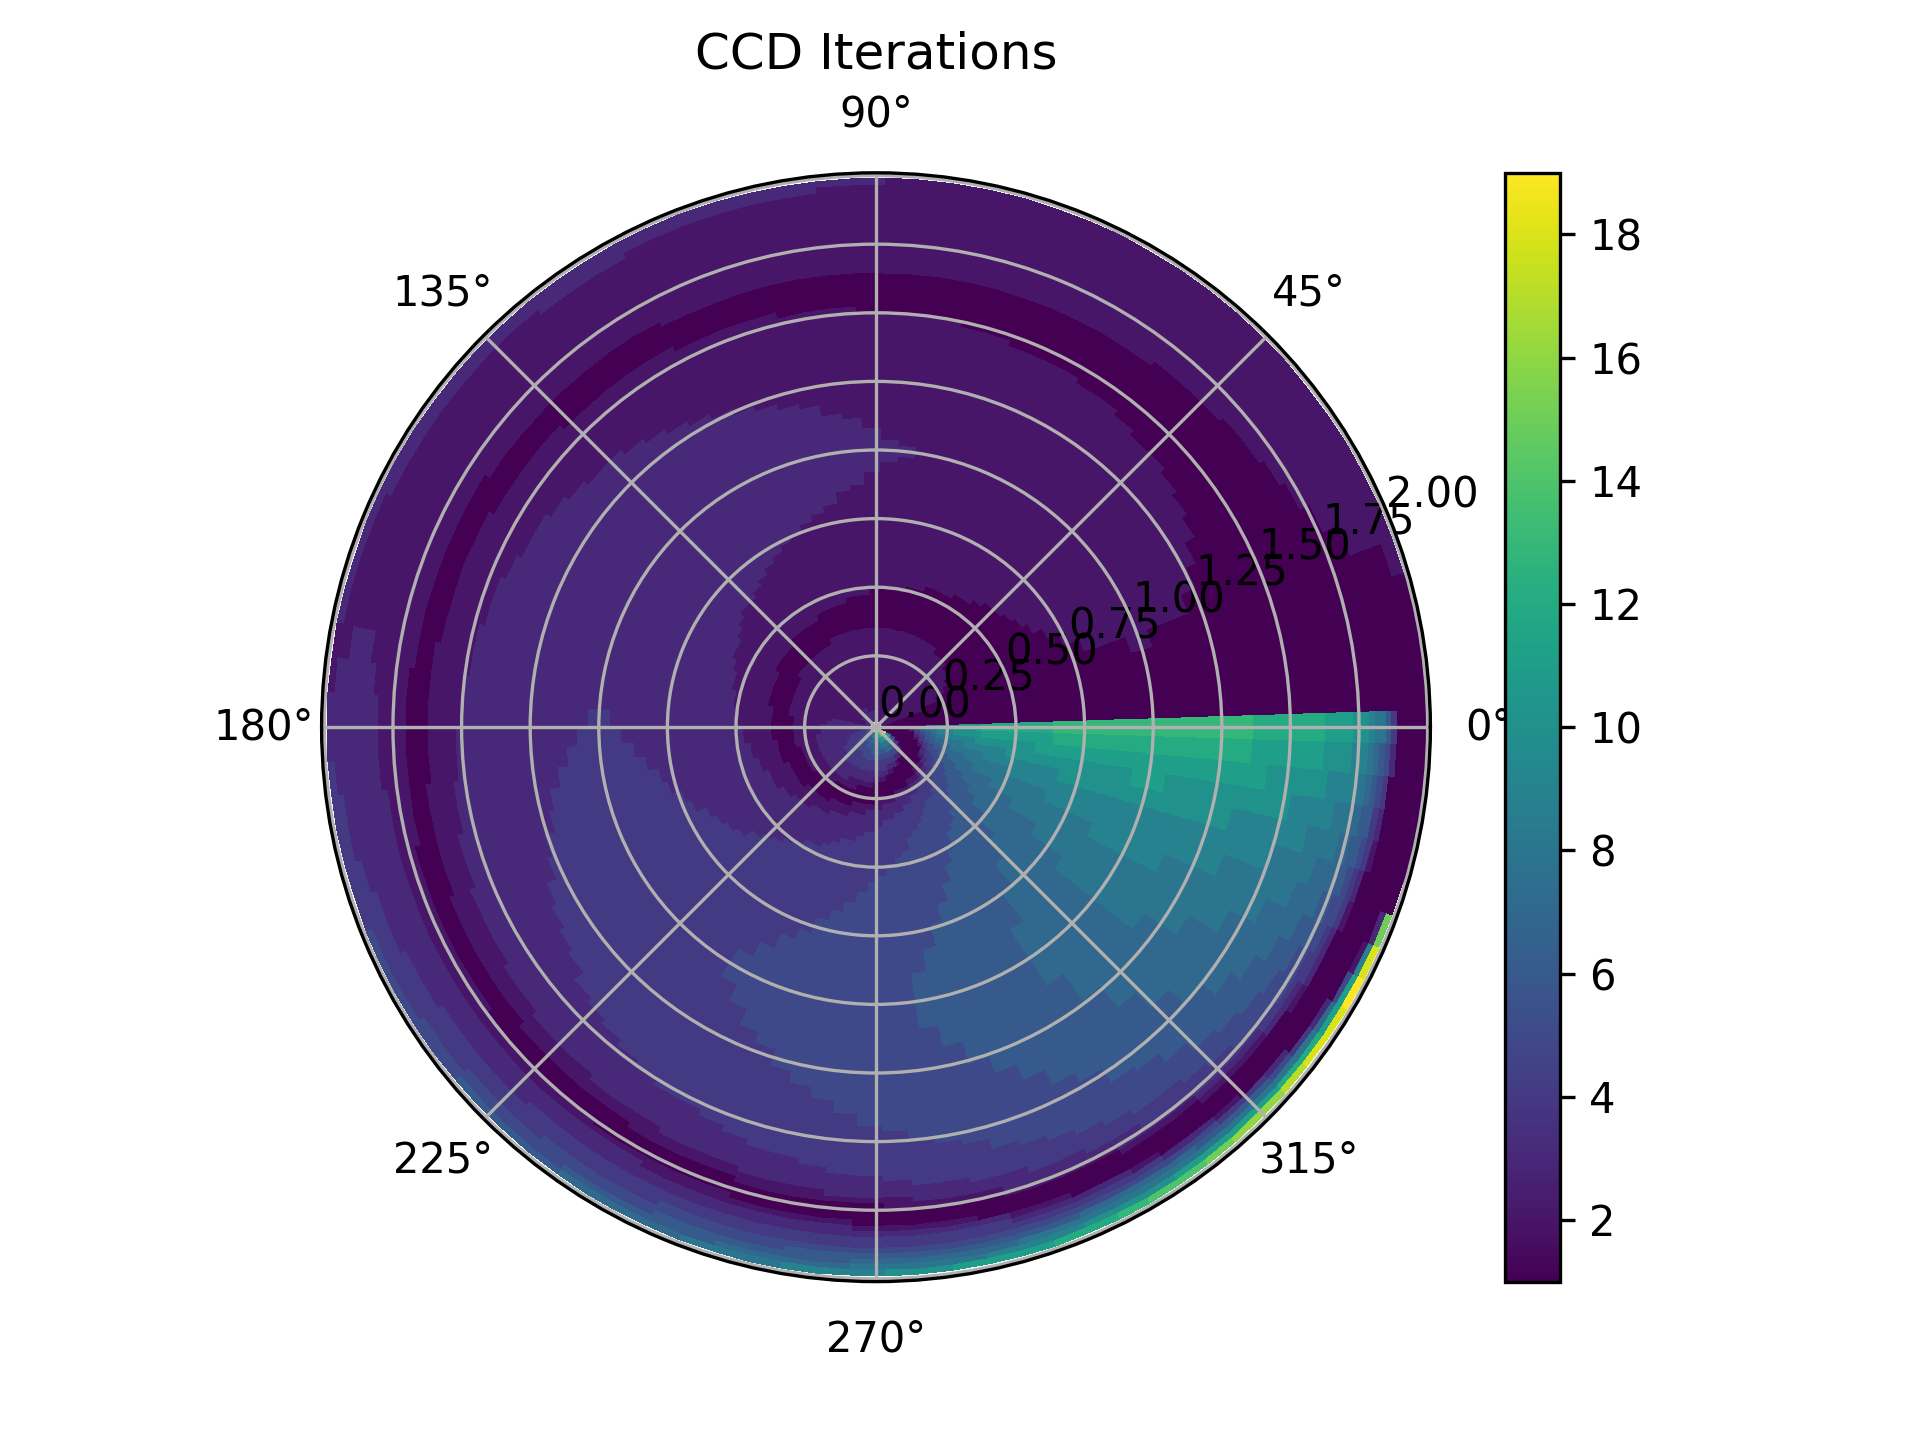
\includegraphics[width=0.31 \linewidth]{figures/background/CCD_2_iteration_heatmap.png}
            \label{fig:CCD_iteration/2}
            }
        \hfill
        \subfloat[$N = 5$]{
            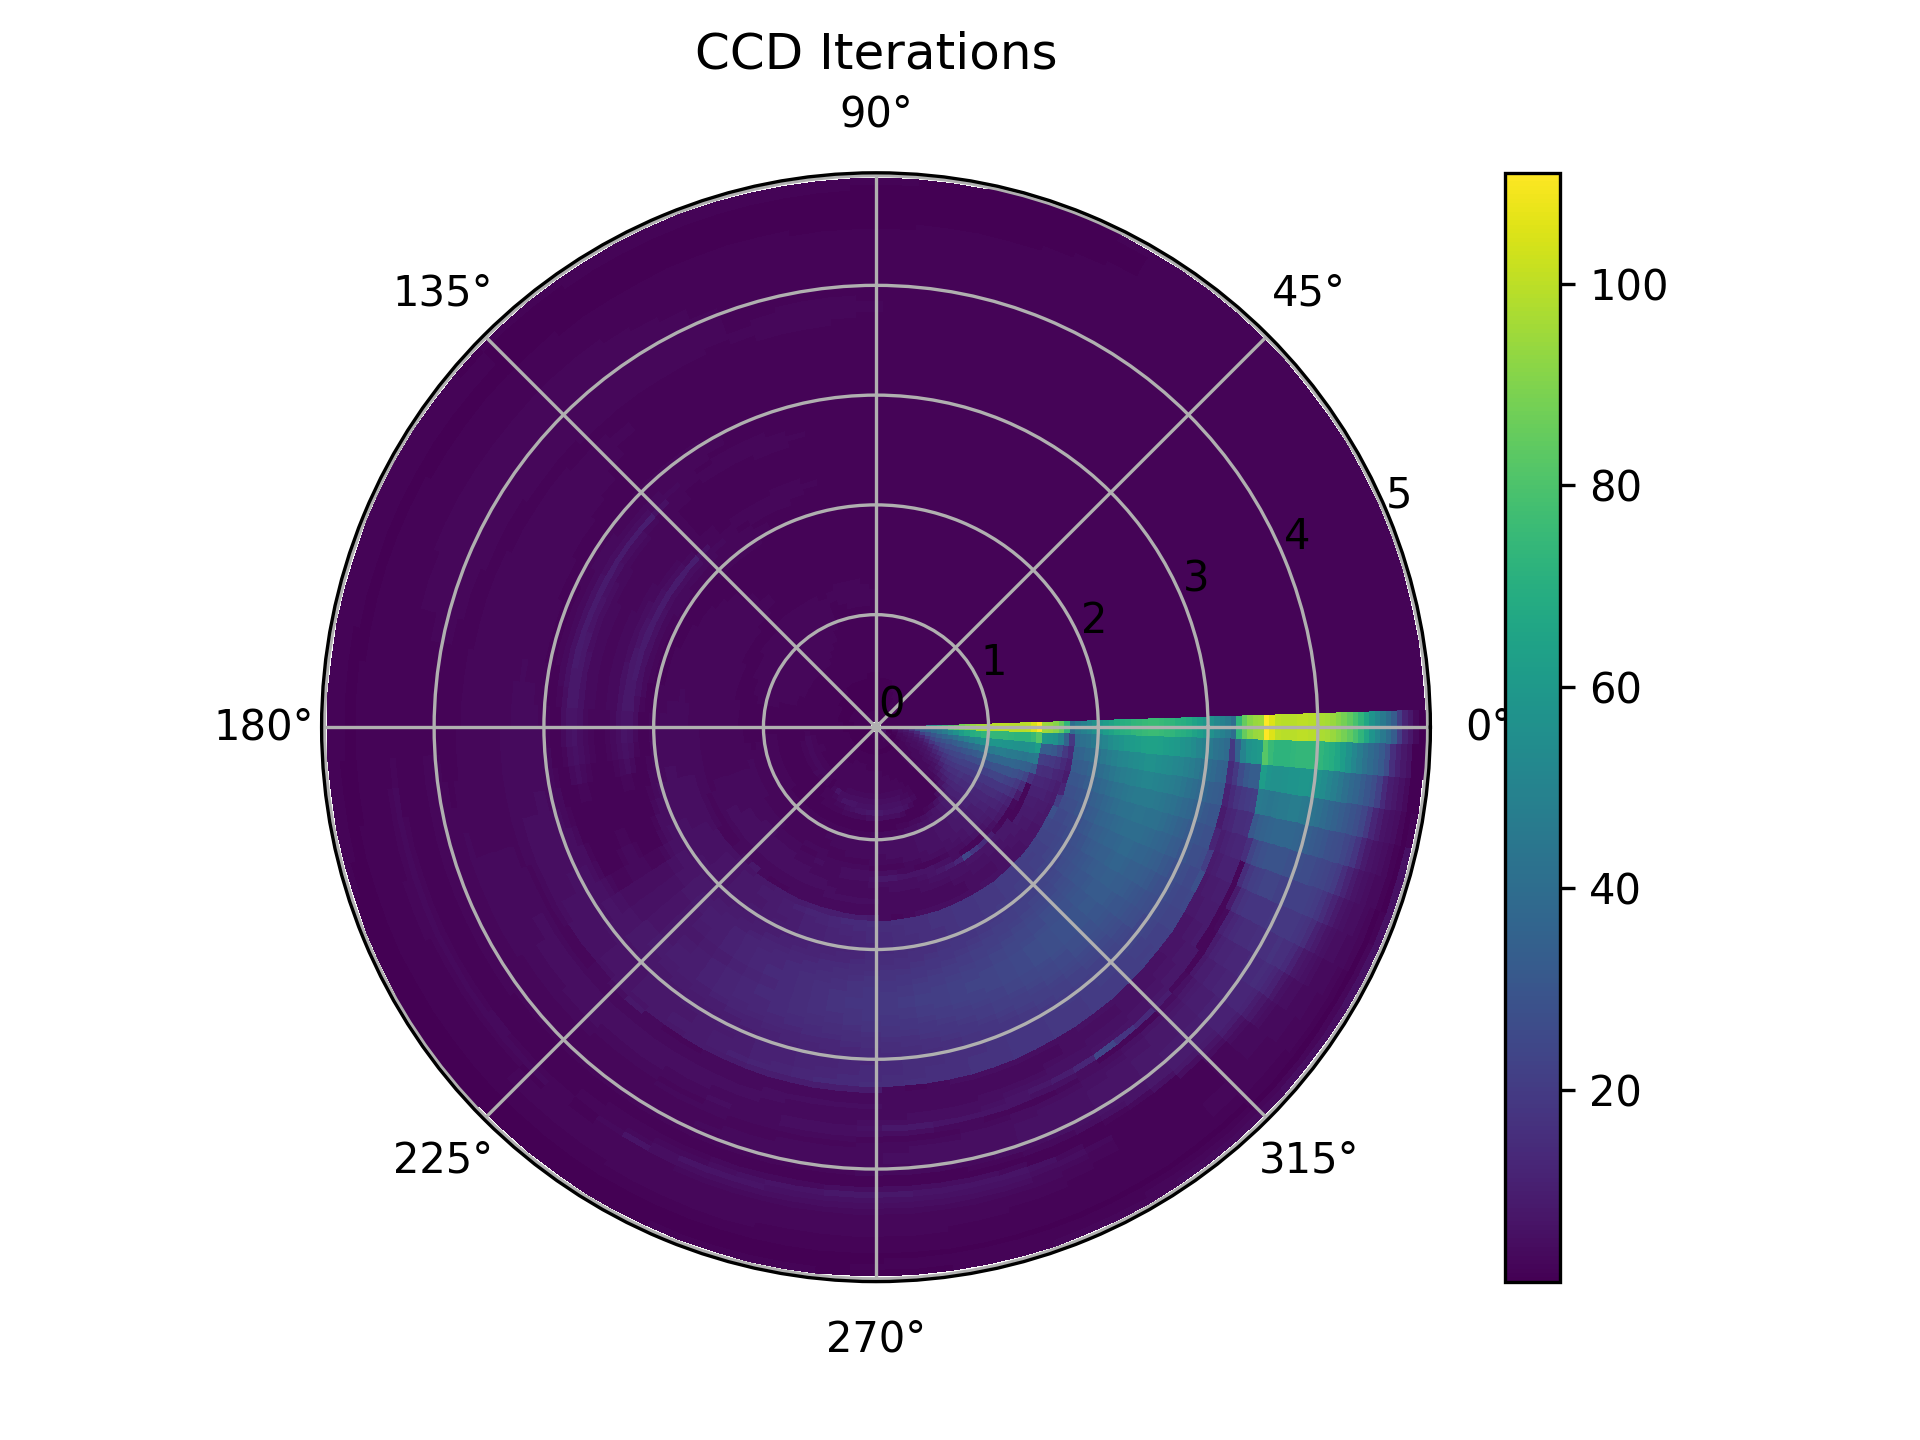
\includegraphics[width=0.31 \linewidth]{figures/background/CCD_5_iteration_heatmap.png}
            \label{fig:CCD_iteration/5}
            }
        \hfill
        \subfloat[$N = 10$]{
            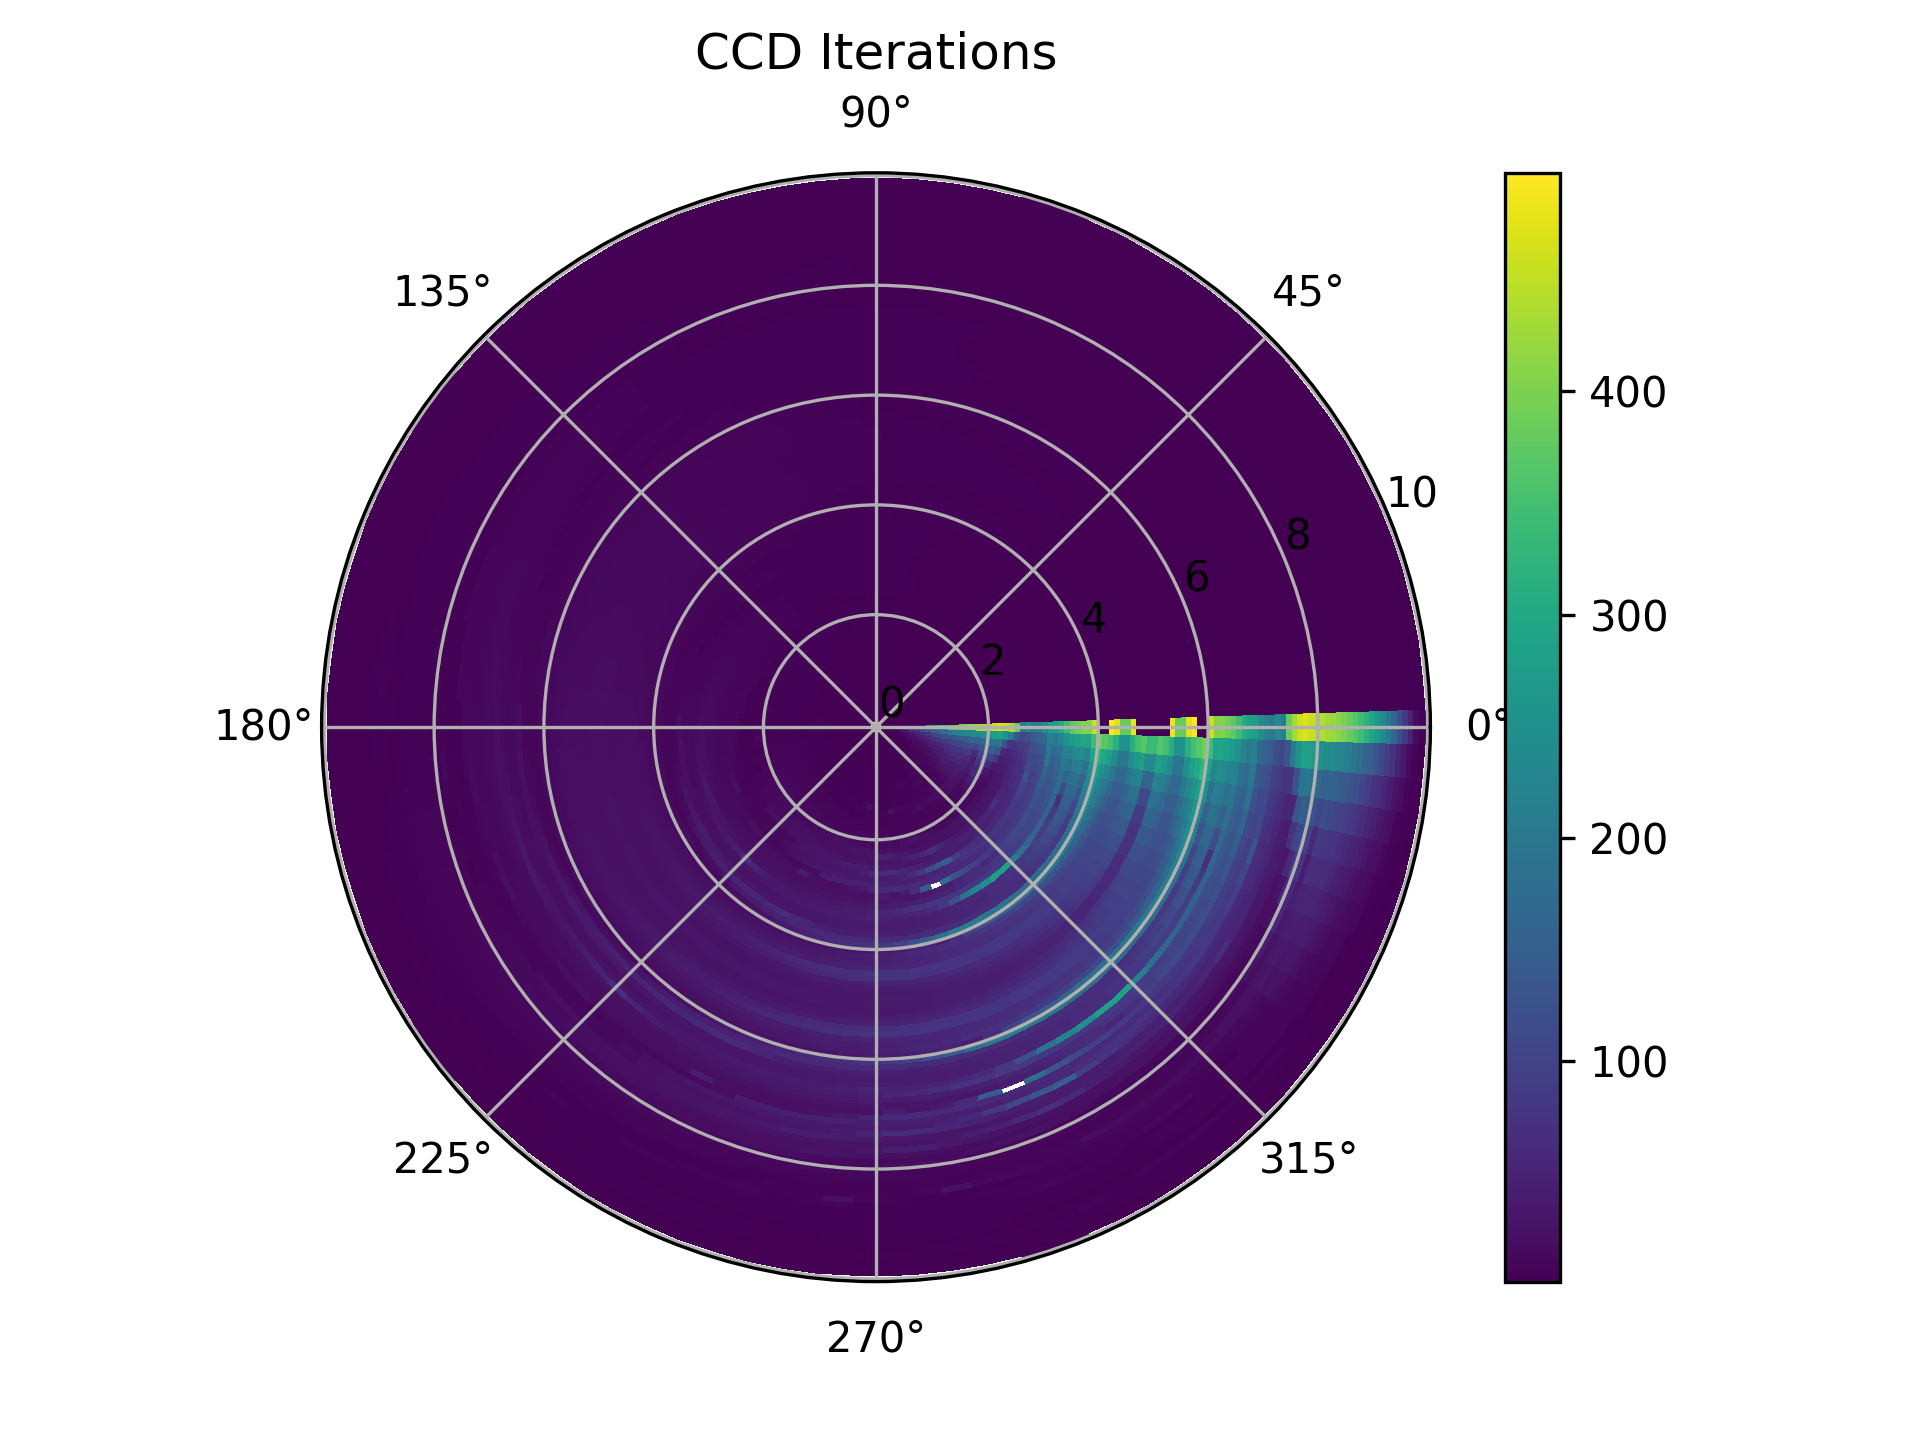
\includegraphics[width=0.31 \linewidth]{figures/background/CCD_10_iteration_heatmap.png}
            \label{fig:CCD_iteration/10}
            }
    \end{center}
    \caption[CCD iteration heatmap]{Heatmap of how many iterations CCD has needed to solve inverse kinematics starting from $[N, 0]$ targeting the middle of each polygon. The maximum budged are 20 times $N$ with a target precision of $0.1$.}
    \label{fig:CCD_iteration}
\end{figure}
\begin{figure}
    \begin{center}
        \subfloat[baseline. number of samples = 32062]{
            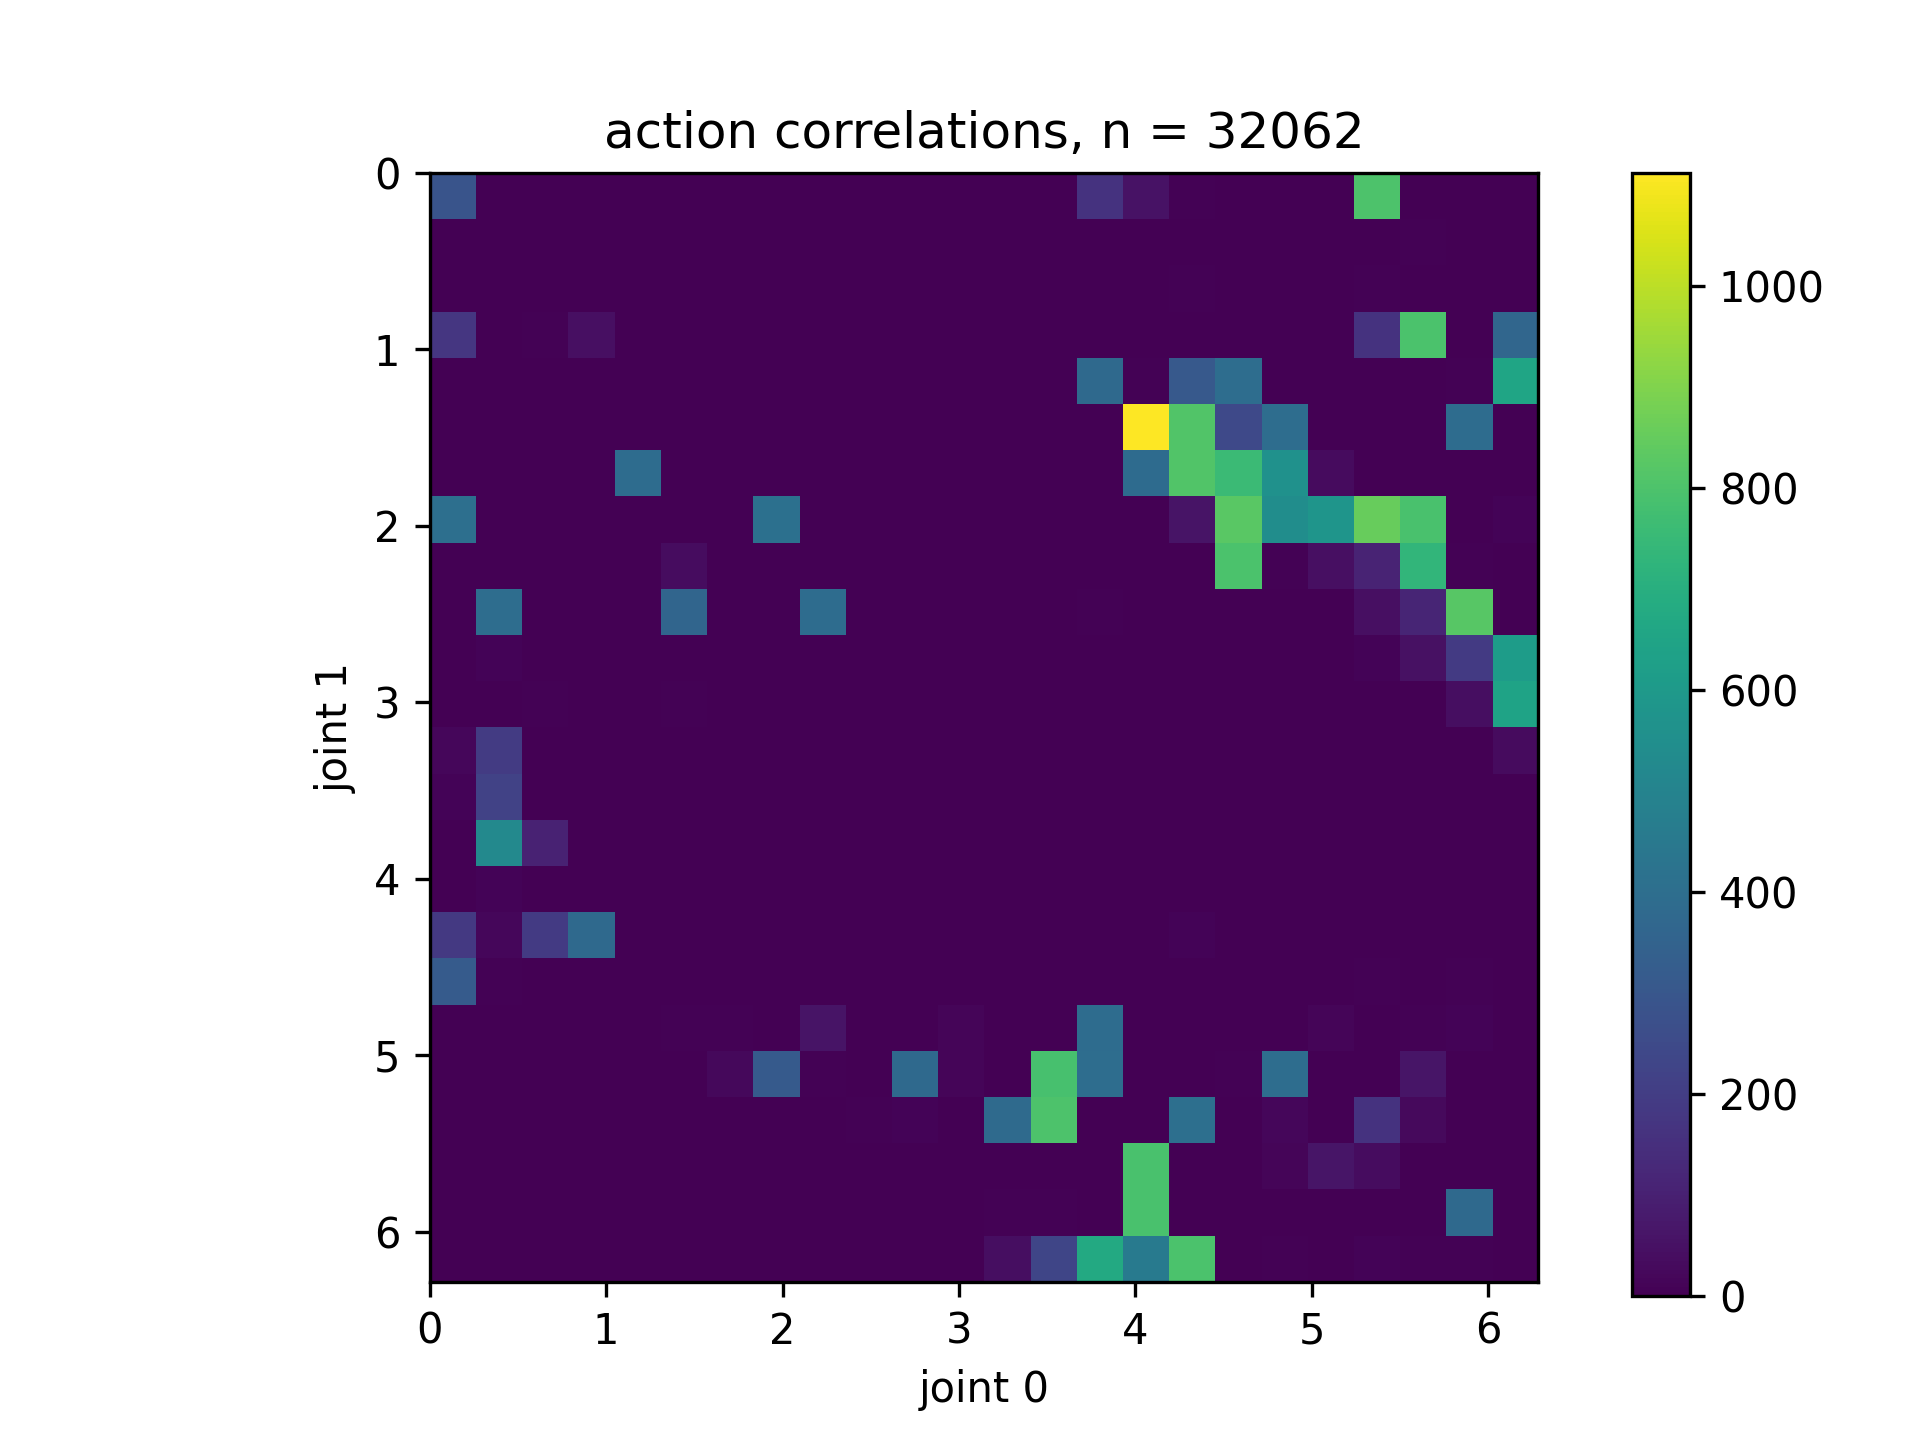
\includegraphics[width=0.23 \linewidth]{figures/experiments/action_correlations_baseline_2_1691621262_5000.png}
            \label{fig:SAC_action_correlation/baseline}
            }
        \hfill
        \subfloat[laten dimension is 2. number of samples = 39992]{
            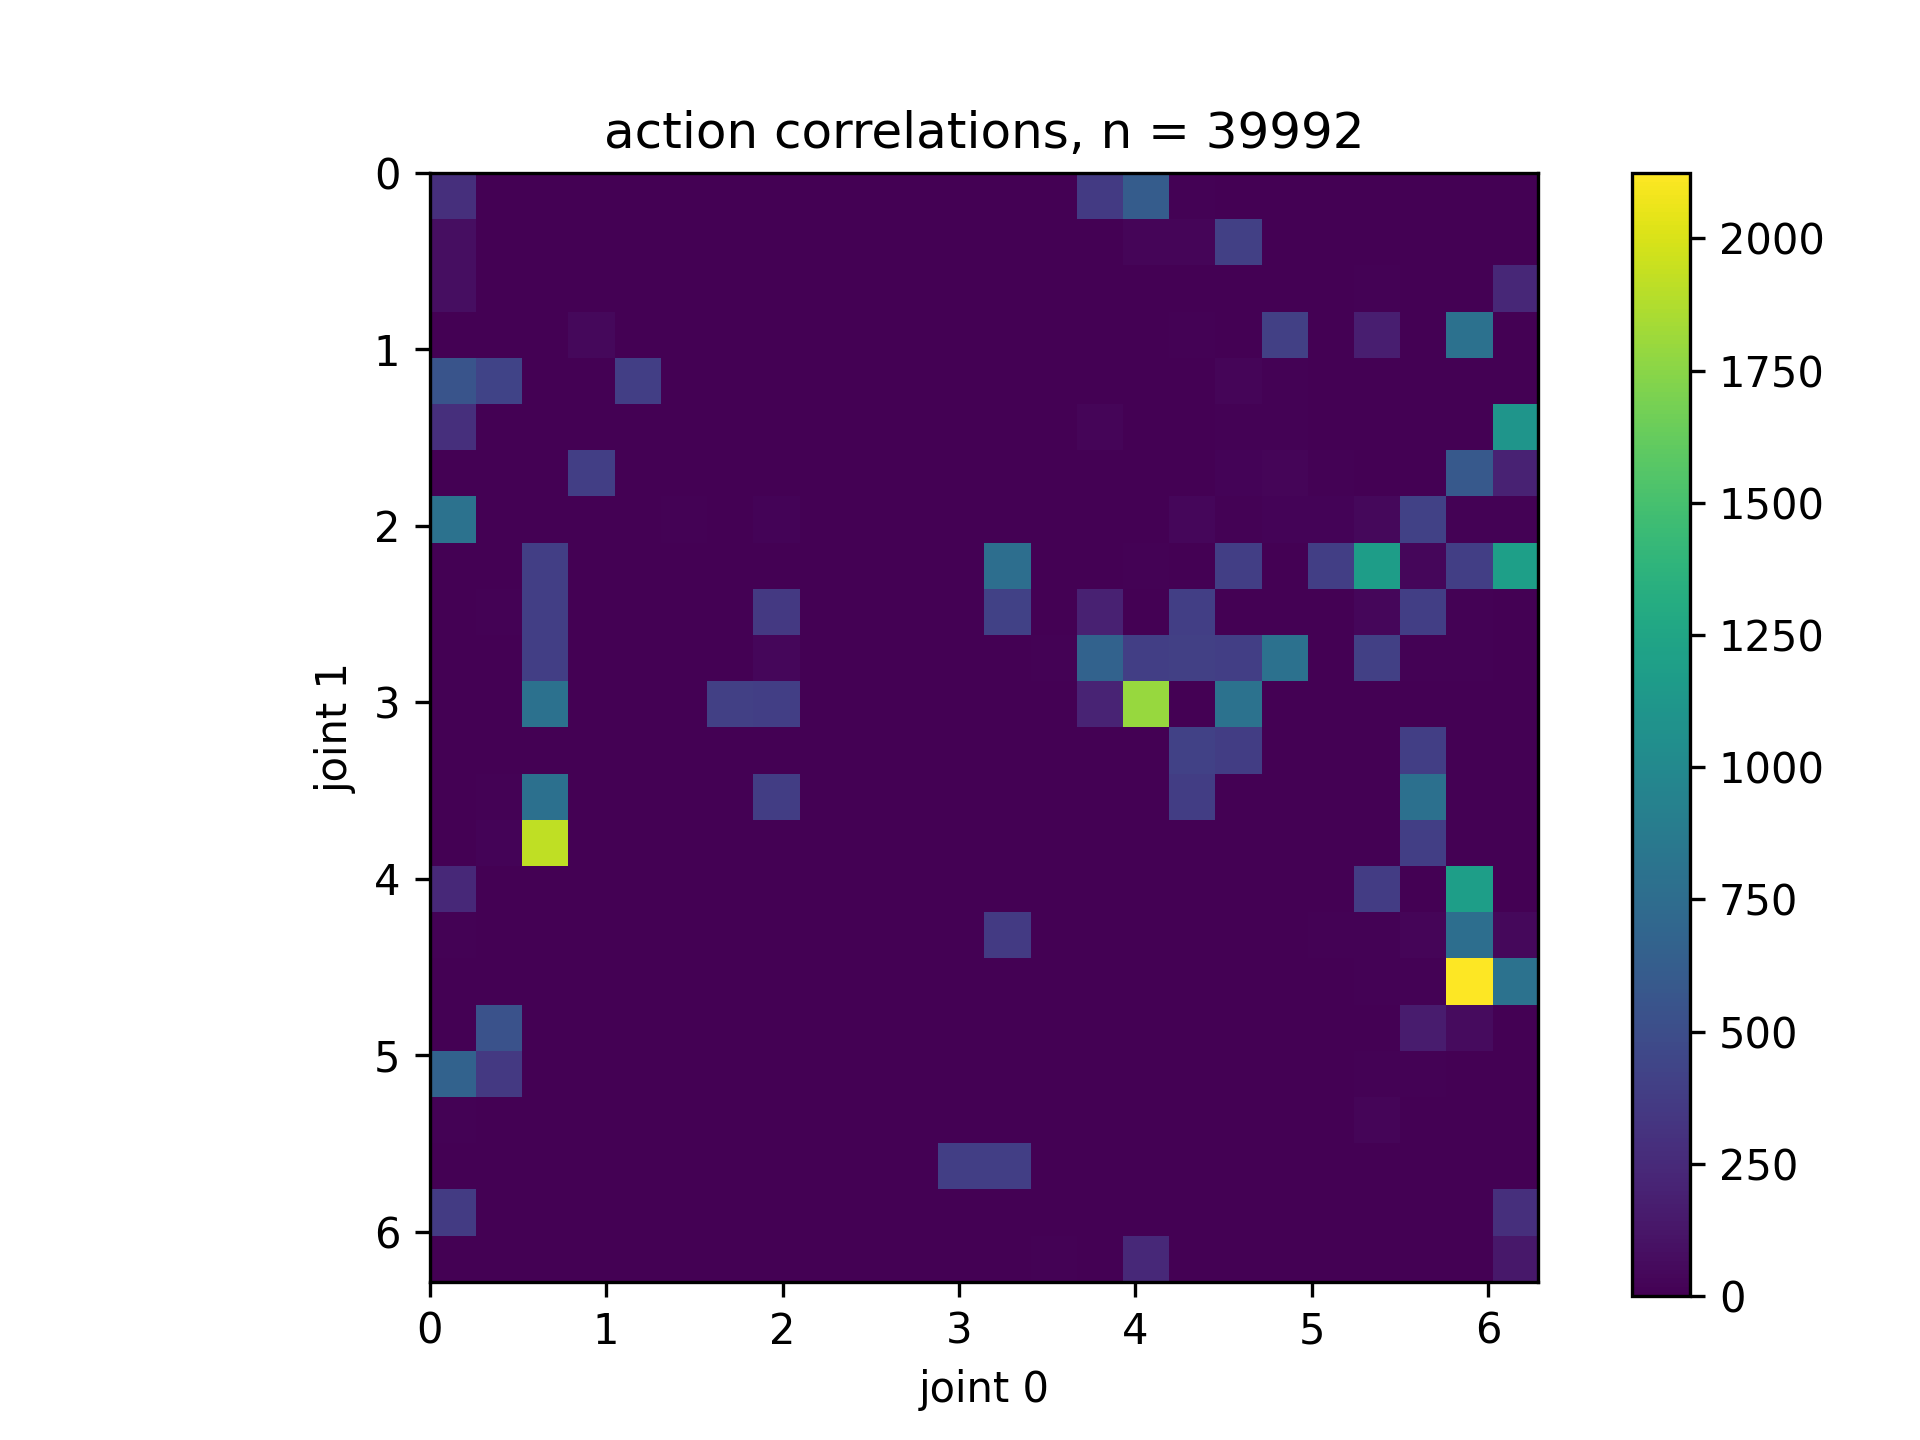
\includegraphics[width=0.23 \linewidth]{figures/experiments/action_correlations_latent_actor_2_2_1693146377_5000.png}
            \label{fig:SAC_action_correlation/latent_2}
            }
        \hfill
        \subfloat[laten dimension is 4. number of samples = 30810]{
            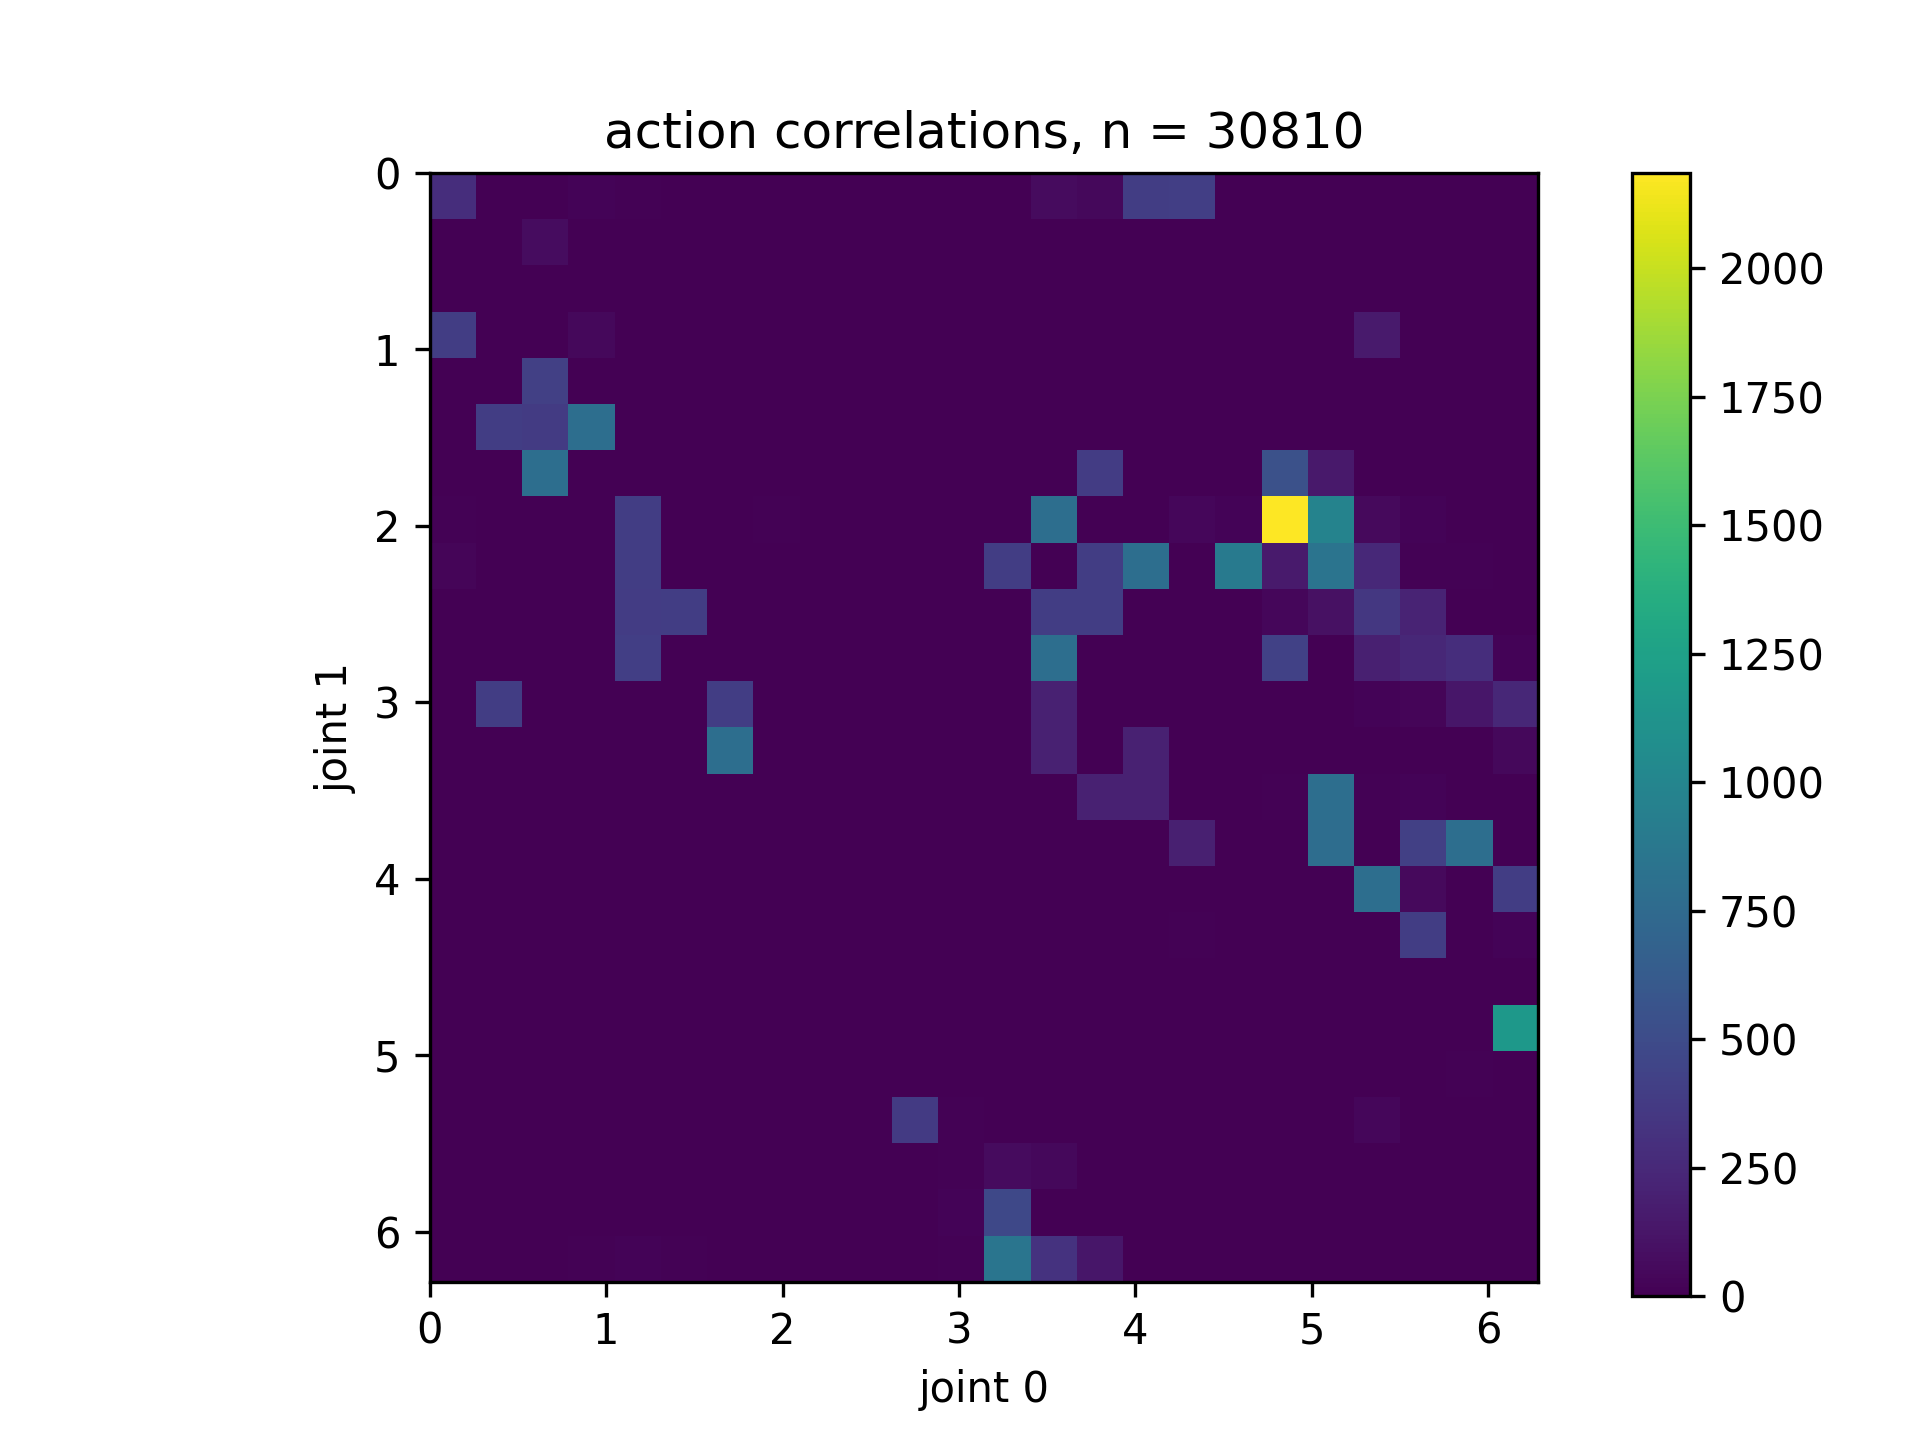
\includegraphics[width=0.23 \linewidth]{figures/experiments/action_correlations_latent_actor_4_2_1693063115_5000.png}
            \label{fig:SAC_action_correlation/latent_4}
            }
        \hfill
        \subfloat[laten dimension is 8. number of samples = 33247]{
            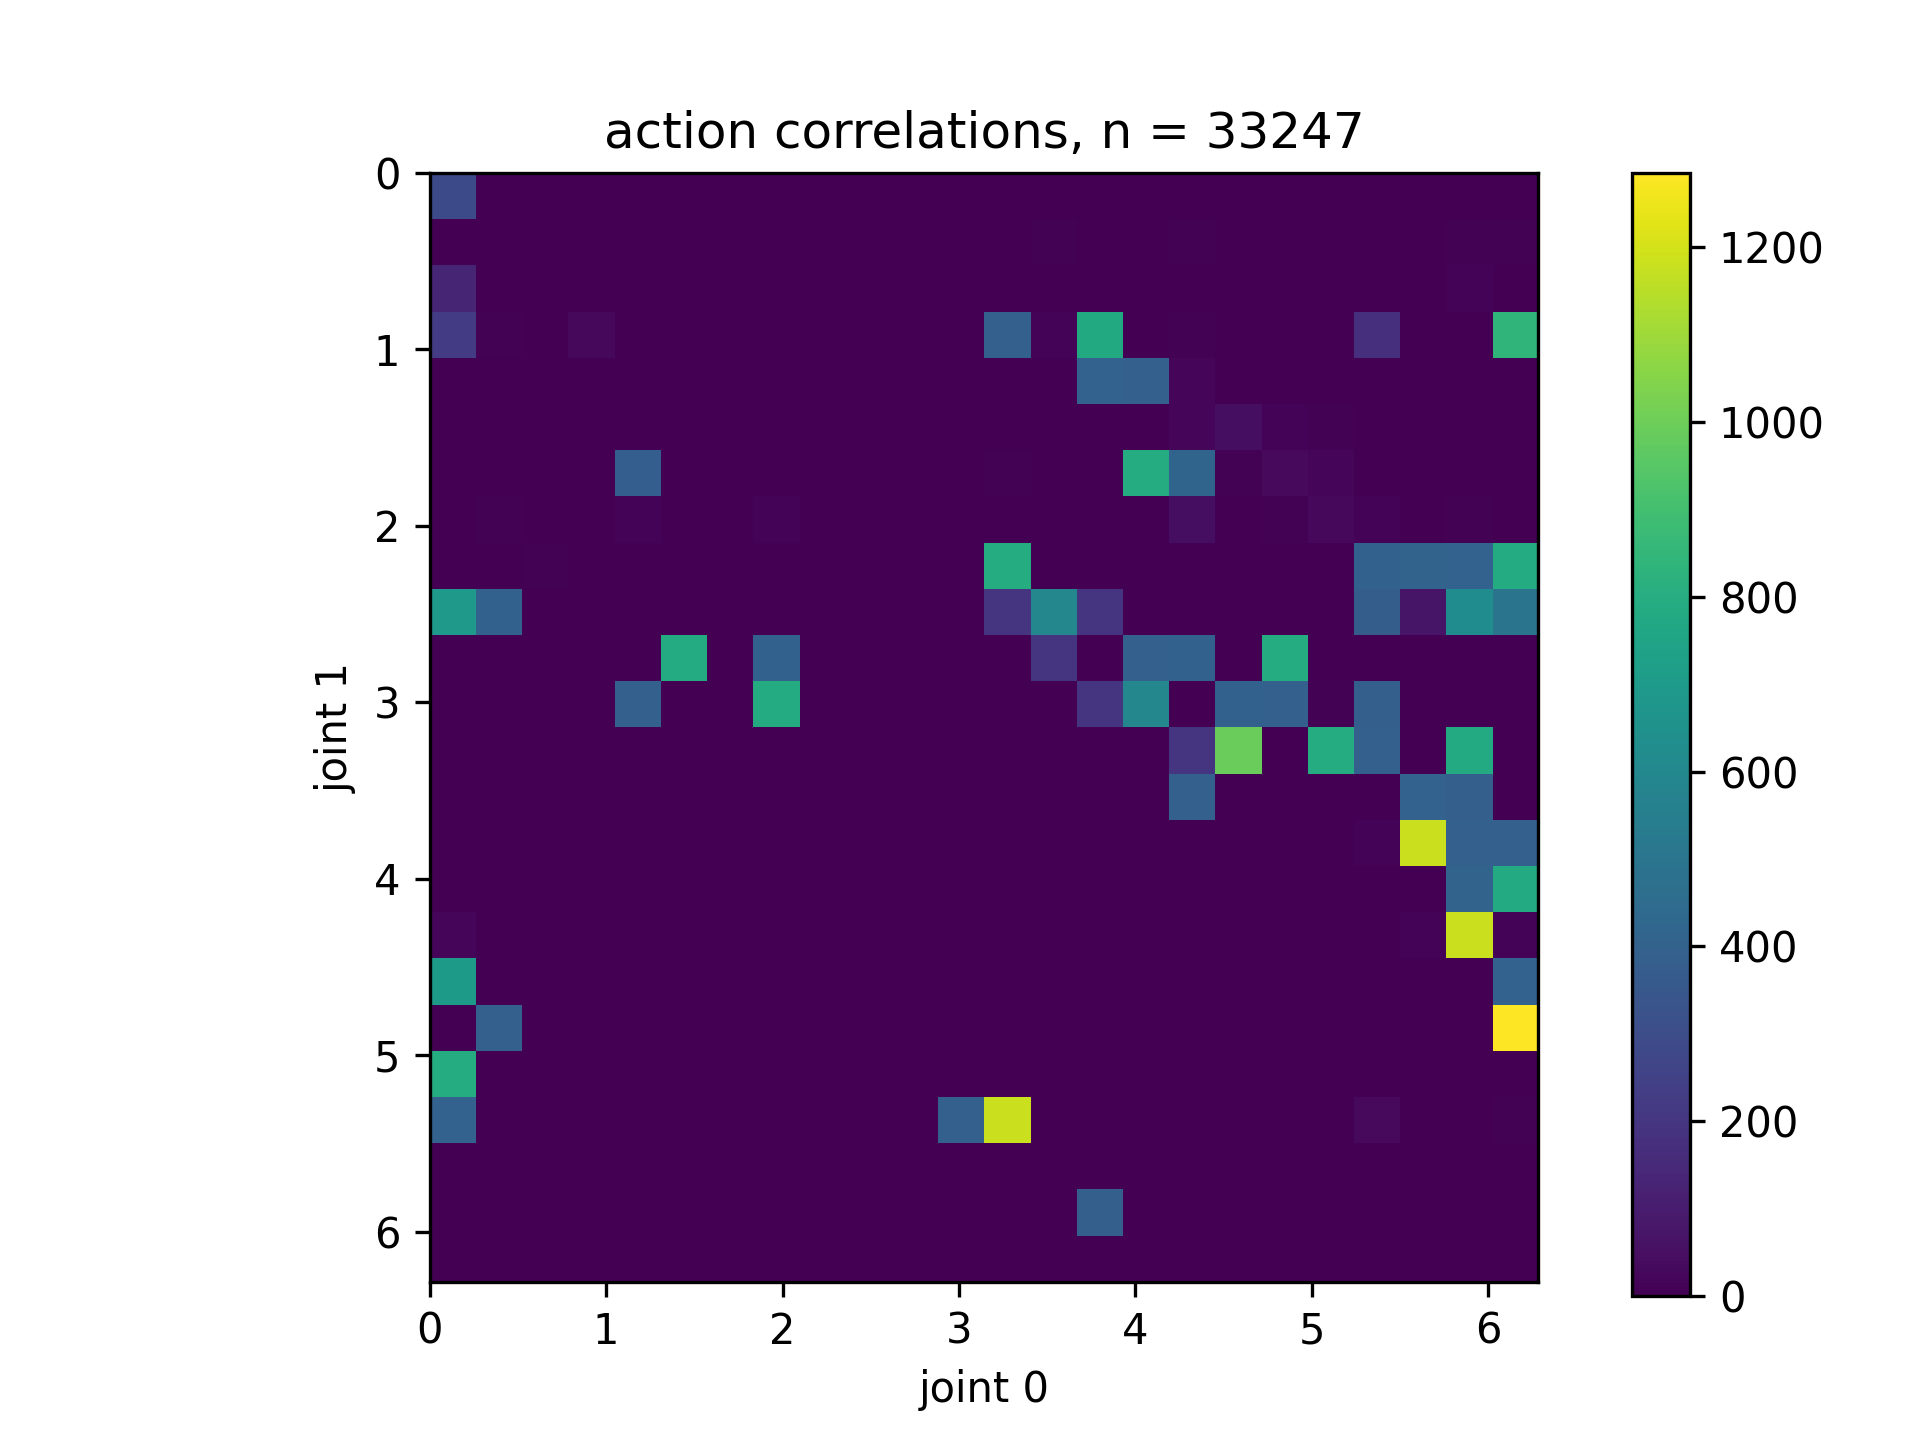
\includegraphics[width=0.23 \linewidth]{figures/experiments/action_correlations_latent_actor_8_2_1691615359_3000.png}
            \label{fig:SAC_action_correlation/latent_8}
            }
    \end{center}
    \caption[action correlation]{Plotted is the state angle correlation of two joints as a 2D histogram. The state angles are sampled from multiple episodes to uniformly sampled target positions. Each bucket can be translated to the amount of angles in one 3D bucket $b$ with limits $b_{0, 0}, b_{0, 1}, b_{1, 0}, b_{1, 1}$. Mathematical speaking: $|b| = |\{q_t | q_t \in [0, 2\pi)^2 \land q_{0, t} \in [b_{0, 0}, b_{0, 1}] \land q_{1, t} \in [b_{1, 0}, b_{1, 1}]\}|$}
    \label{fig:SAC_action_correlation}
\end{figure}


While comparing the CCD with baseline SAC we found a couple of differences those two solvers present.
\begin{itemize}
    \item \textbf{Target Dependence}: By looking deeper into CCD it is clear that its granular performance in a single run is also highly dependent on the given start configuration and target as show in \figref{fig:CCD_iteration}. Note that we talk about the performance of CCD as the number of iterations needed to reach the desired target position. If we now look into the steps needed to reach the desired target position of SAC we can seed that while increasing the number of joints we are increasingly often capped by the maximum number of iterations than ending the episode by reaching the target. One possible reason is teased by \figref{fig:SAC_baseline_inference_trajectory}. Here we were able to see that the agents behavior sometimes collapses as it is about to reach the target but after failing very closely the end-effector moves rapidly towards the origin and never coming as close as before to the desired target position. This observation is supported by \figref{fig:SAC_baseline_min_distance_step} where the minimal distance to the target can be found almost all of the time at around 50 or less steps in the episode. One reason why the agent struggles to reach the target with a increasing amount of joints could be the constant threshold to end an episode of 0.1 euclidean distance between end-effector and target position. As we increase the number of joints the area where the end-effector position ends an episode decreases due to $A = \pi N^2$ quadratically which makes it even harder to reach the position while increasing $N$. Against this argument stands that the robot arm is capable to perform more precise movements or even reducing the problem further down. One strategy could position joint 1 to $N - 2$ so the last two joints are able to reach the target and let do joint $N - 1$ to $N$ do the precise work. But why is the agent failing with a high margin after it went so close towards the target? An explanation could be that the agent is reaching a target very often dependent on the actual target position and has no opportunity to learn from those experiences. On the other hand are the  extended episode length and the increasing failure rate as in \tabref{tab:SAC_solved_ratio}.
    \item \textbf{Solutions}: While having a deeper look into the solutions how SAC and CCD solve Inverse Kinematics we can observe a vast difference in the state angle distribution Comparing \figref{fig:dataset_action_correlation} to \figref{fig:SAC_action_correlation/baseline}. While in \figref{fig:dataset_action_correlation} the state angles to reach the target distribution are rhombus shaped the state angle plot in \figref{fig:SAC_action_correlation/baseline} is way more scattered. This change is also observable while looking deeper into the chosen trajectory. 
\end{itemize}

Note that this is only an qualitative comparison because CCD has the full action space on its disposal while SAC is limited to -1 to one because of the action normalizer at the back of SAC. Although scaling the tanh output up to a span of $2\pi$ or higher is not the perfect solution because SAC could find multiple actions for the same action outcome. It could also interfere with computing the probability of $\log(\pi_\theta(a|s))$.

The presented decrease in the SAC performance in \figref{fig:SAC_baseline} could be also explained because of the linear increase of complexity of the observation space since $S \subset \mathbb{R}^{4+N}$. To counter the increase of complexity some could also increase the number of hidden layer or neurons per layer and have a closer look into neural architecture search. Another way to maybe proof this theory could be the application of Neural-Evolution-of-Augmented-Topologies short NEAT. This algorithm finds the smallest possible architecture to conquer a given task. Given the provided background information we assume the found neural architecture increases in complexity while increasing $N$.

Comparing RL with SAC we already described the end-effector movements in \chapref{chap:experiments}. With the current training settings it is clear that SAC is clearly not the better solutions than a more standard approach like SAC as we can see for the solved rar

\begin{figure}
    \begin{center}
        \subfloat[$N = 2$]{
            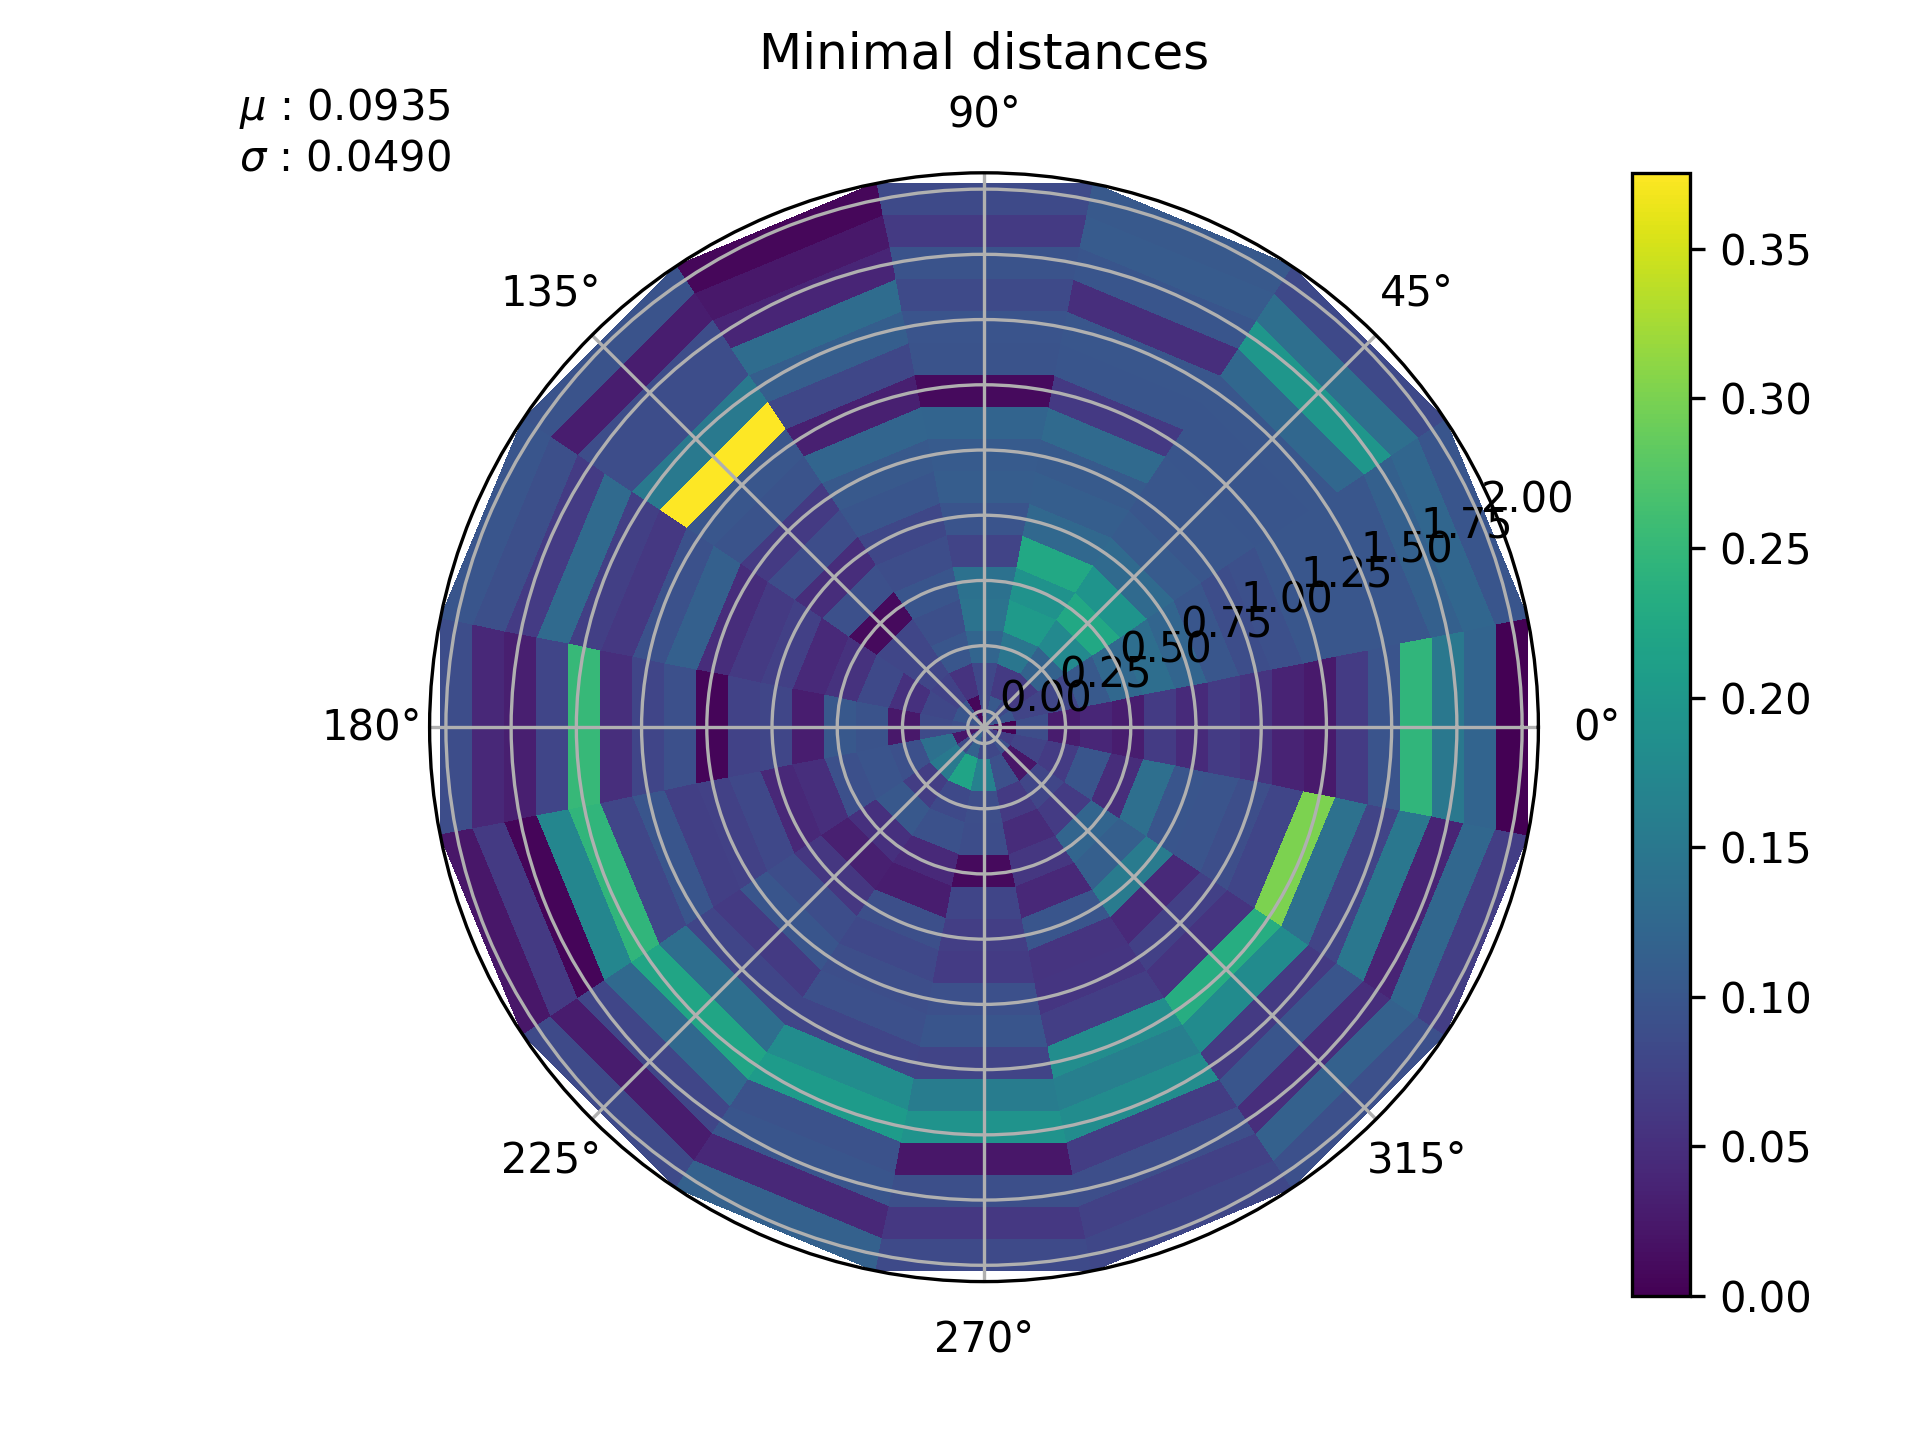
\includegraphics[width=0.31 \linewidth]{figures/experiments/Minimal_distances_baseline_2_1691621262_5000.png}
            \label{fig:SAC_baseline_min_distances/2}
            }
        \hfill
        \subfloat[$N = 5$]{
            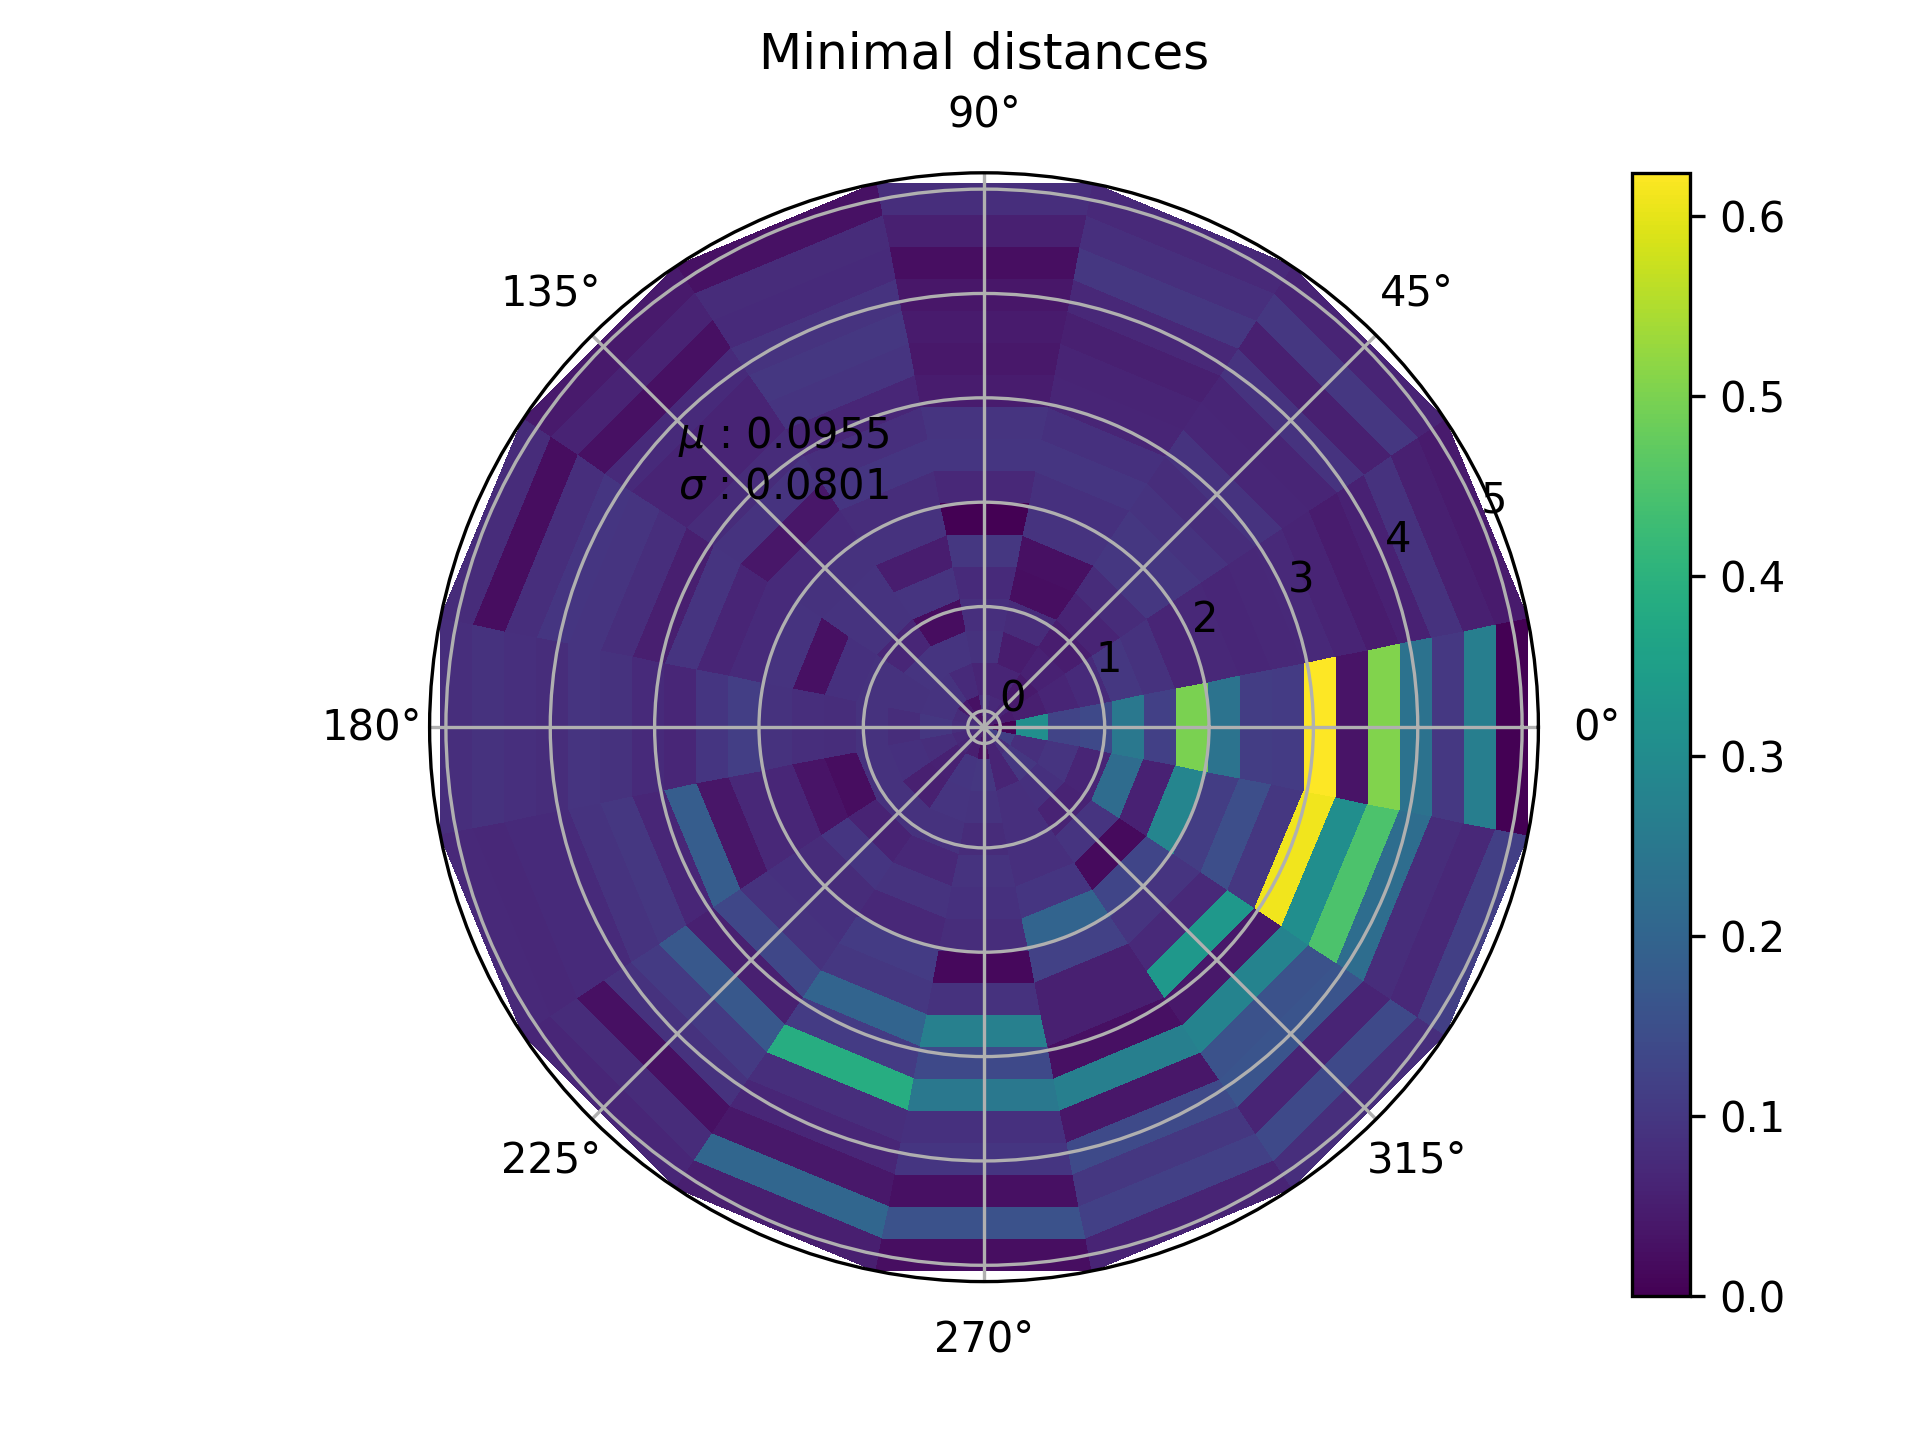
\includegraphics[width=0.31 \linewidth]{figures/experiments/Minimal_distances_baseline_5_1691621331_5000.png}
            \label{fig:SAC_baseline_min_distances/5}
            }
        \hfill
        \subfloat[$N = 10$]{
            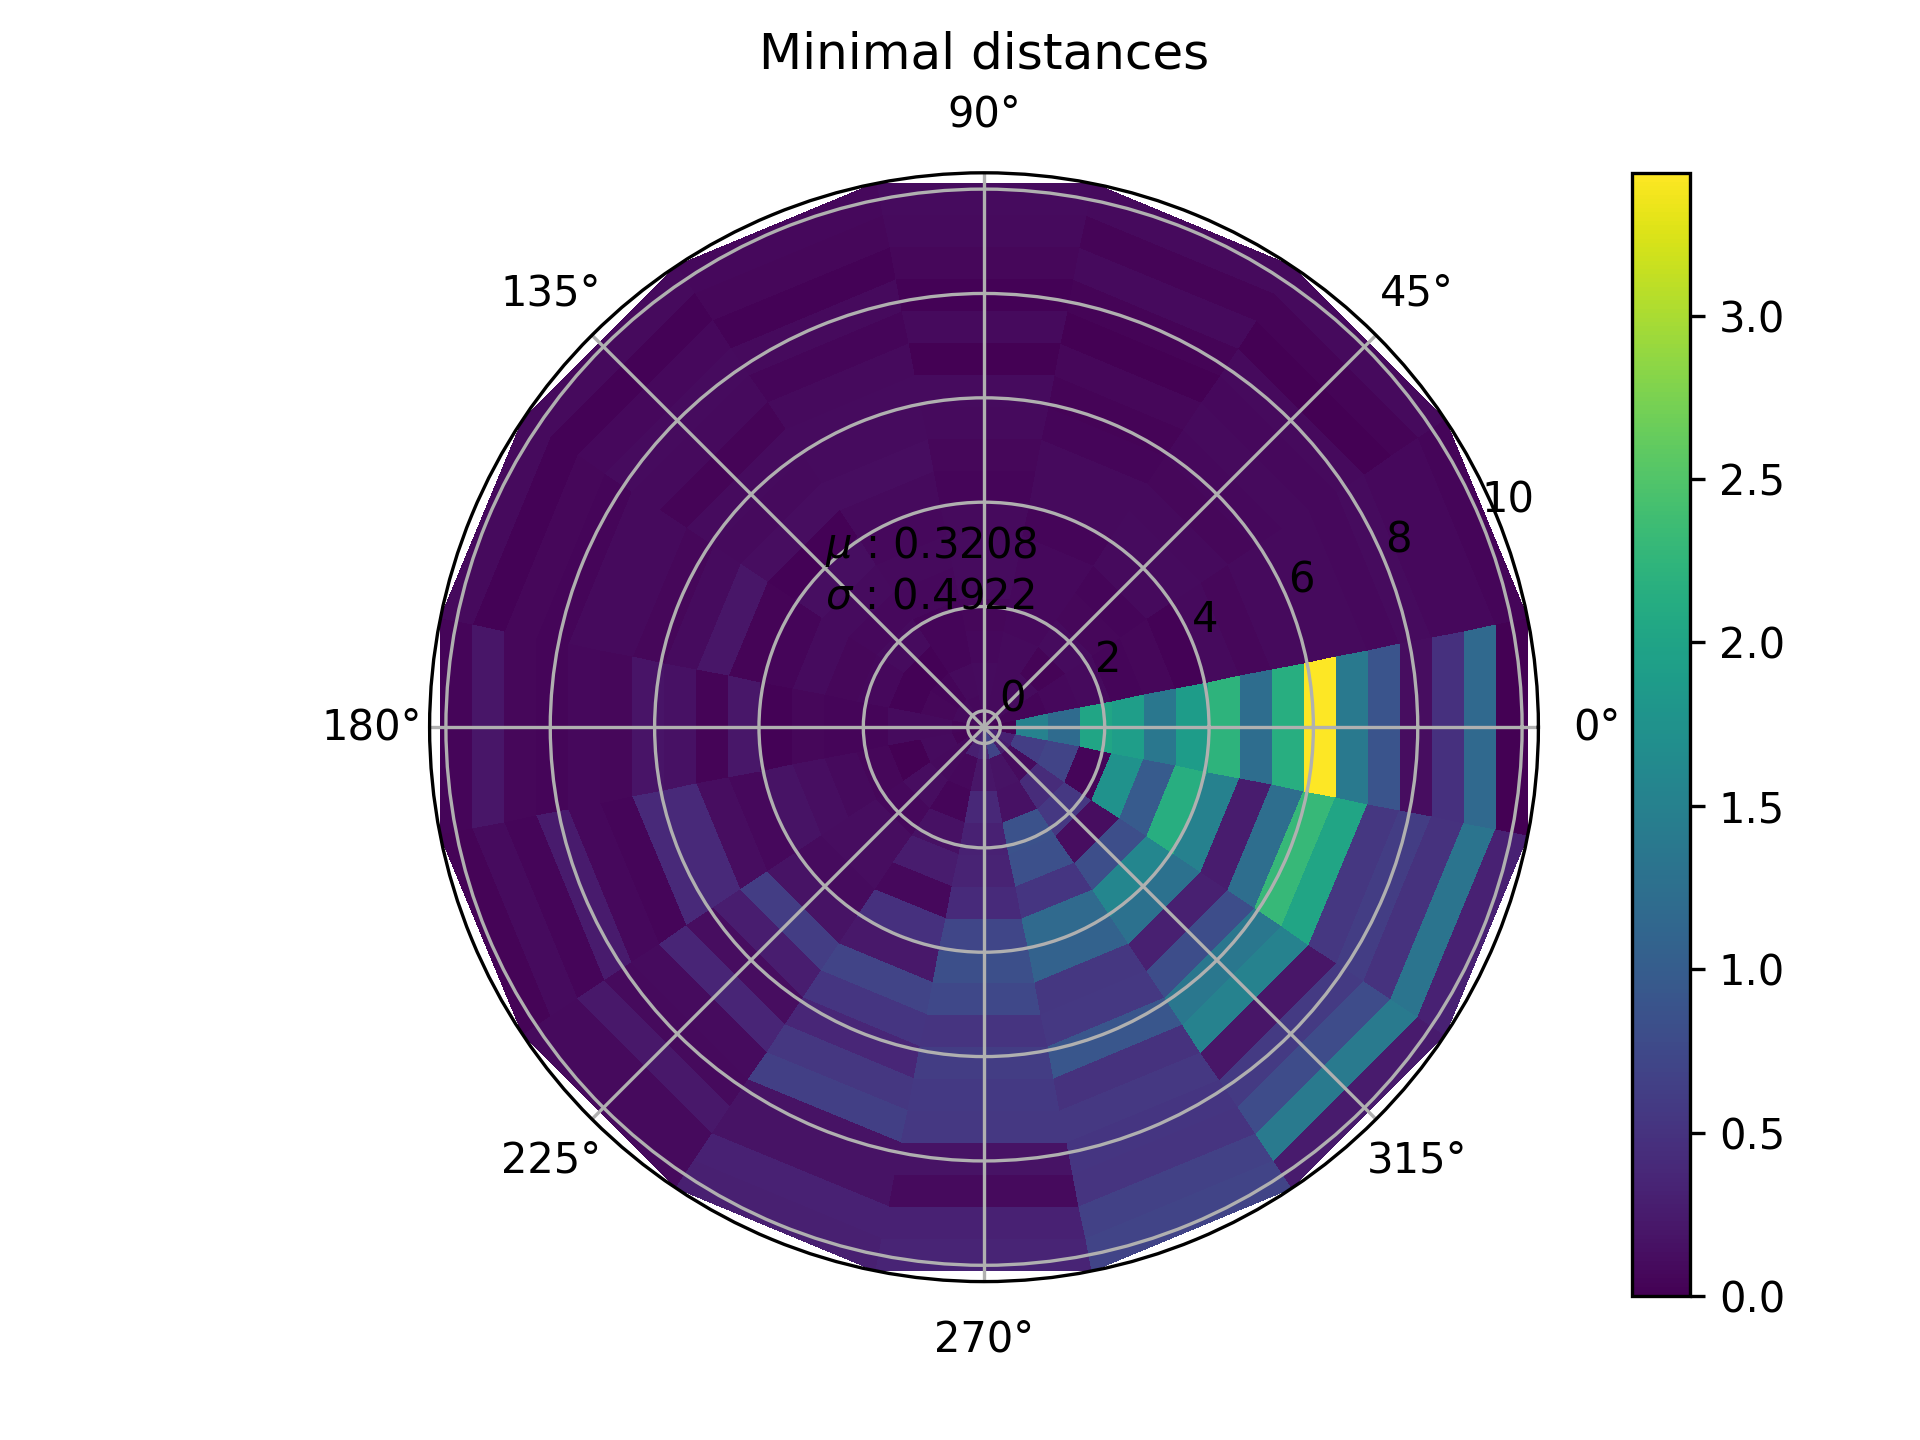
\includegraphics[width=0.31 \linewidth]{figures/experiments/Minimal_distances_baseline_10_1691618968_5000.png}
            \label{fig:SAC_baseline_min_distances/10}
            }
    \end{center}
    \caption[SAC min distance heatmap]{Minimal distance to a target during inference starting from $[N , 0]$ and targeting the middle of each polygon.}
    \label{fig:SAC_baseline_min_distances}
\end{figure}

\begin{table}
    \begin{center}
        \begin{tabular}{ l l | l l l l l}
        experiment series           & $N$                   & 2    & 5    & 10   & 15   & 20   \\
        \hline
        \hline
        \textit{baseline}           & $\mathfrak{S}$        & 0.73 & 0.83 & 0.57 & 0.42 & 0.30 \\
                                    & max eval $\bar{R_t}$  & 0.09 & 0.10 & 0.32 & 0.74 & 0.82 \\
        \hline
        \textit{latent 2}           & $\mathfrak{S}$        & 0.66 & 0.78 & 0.33 & 0.04 &      \\
                                    & max eval $\bar{R_t}$  & 0.11 & 0.15 & 0.83 & 3.62 &      \\
        \hline
        \textit{latent 4}           & $\mathfrak{S}$        & 0.76 & 0.84 & 0.54 &      &      \\
                                    & max eval $\bar{R_t}$  & 0.09 & 0.09 & 0.50 &      &      \\
        \hline
        \textit{latent 8}           & $\mathfrak{S}$        & 0.72 & 0.88 & 0.22 &      &      \\
                                    & max eval $\bar{R_t}$  & 0.09 & 0.08 & 2.97 &      &      \\
        \hline
        \textit{latent imitation}   & $\mathfrak{S}$        & 0.85 & 0.85 & ?    &      &      \\
                                    & max eval $\bar{R_t}$  & ?    & ?    & ?    &      &      \\
        \hline
        \textit{super distance}     & $\mathfrak{S}$        & 0.62 & 0.60 & 0.53 &      &      \\
                                    & max eval $\bar{R_t}$  & ?    & ?    & ?    &      &      \\
        \hline
        \textit{super imitation}    & $\mathfrak{S}$        & ?    & ?    & ?    &      &      \\
                                    & max eval $\bar{R_t}$  & ?    & ?    & ?    &      &      \\
    \end{tabular}
    \end{center}
    \caption[SAC Solved ratio]{Solved ratio $\mathfrak{S}$ and closest distance to target during one episode as known as the maximum reward during one episode for one target position, for all SAC experiments starting at $[N, 0]$ and targeting the same targets as in \figref{fig:SAC_baseline_min_distances} with a maximal budged of 400 steps. Those are examples from individual experiments all from epoch 3000. For more details which experiments please have a look into the figures directory. The suffix of each png describes where to find the experiment. For a closer inspection of how the individual models perform over the evaluation please refer to \chapref{chap:appendix}}
    \label{tab:SAC_solved_ratio}
\end{table}

\begin{figure}
    \begin{center}
        \subfloat[$N = 2$]{
            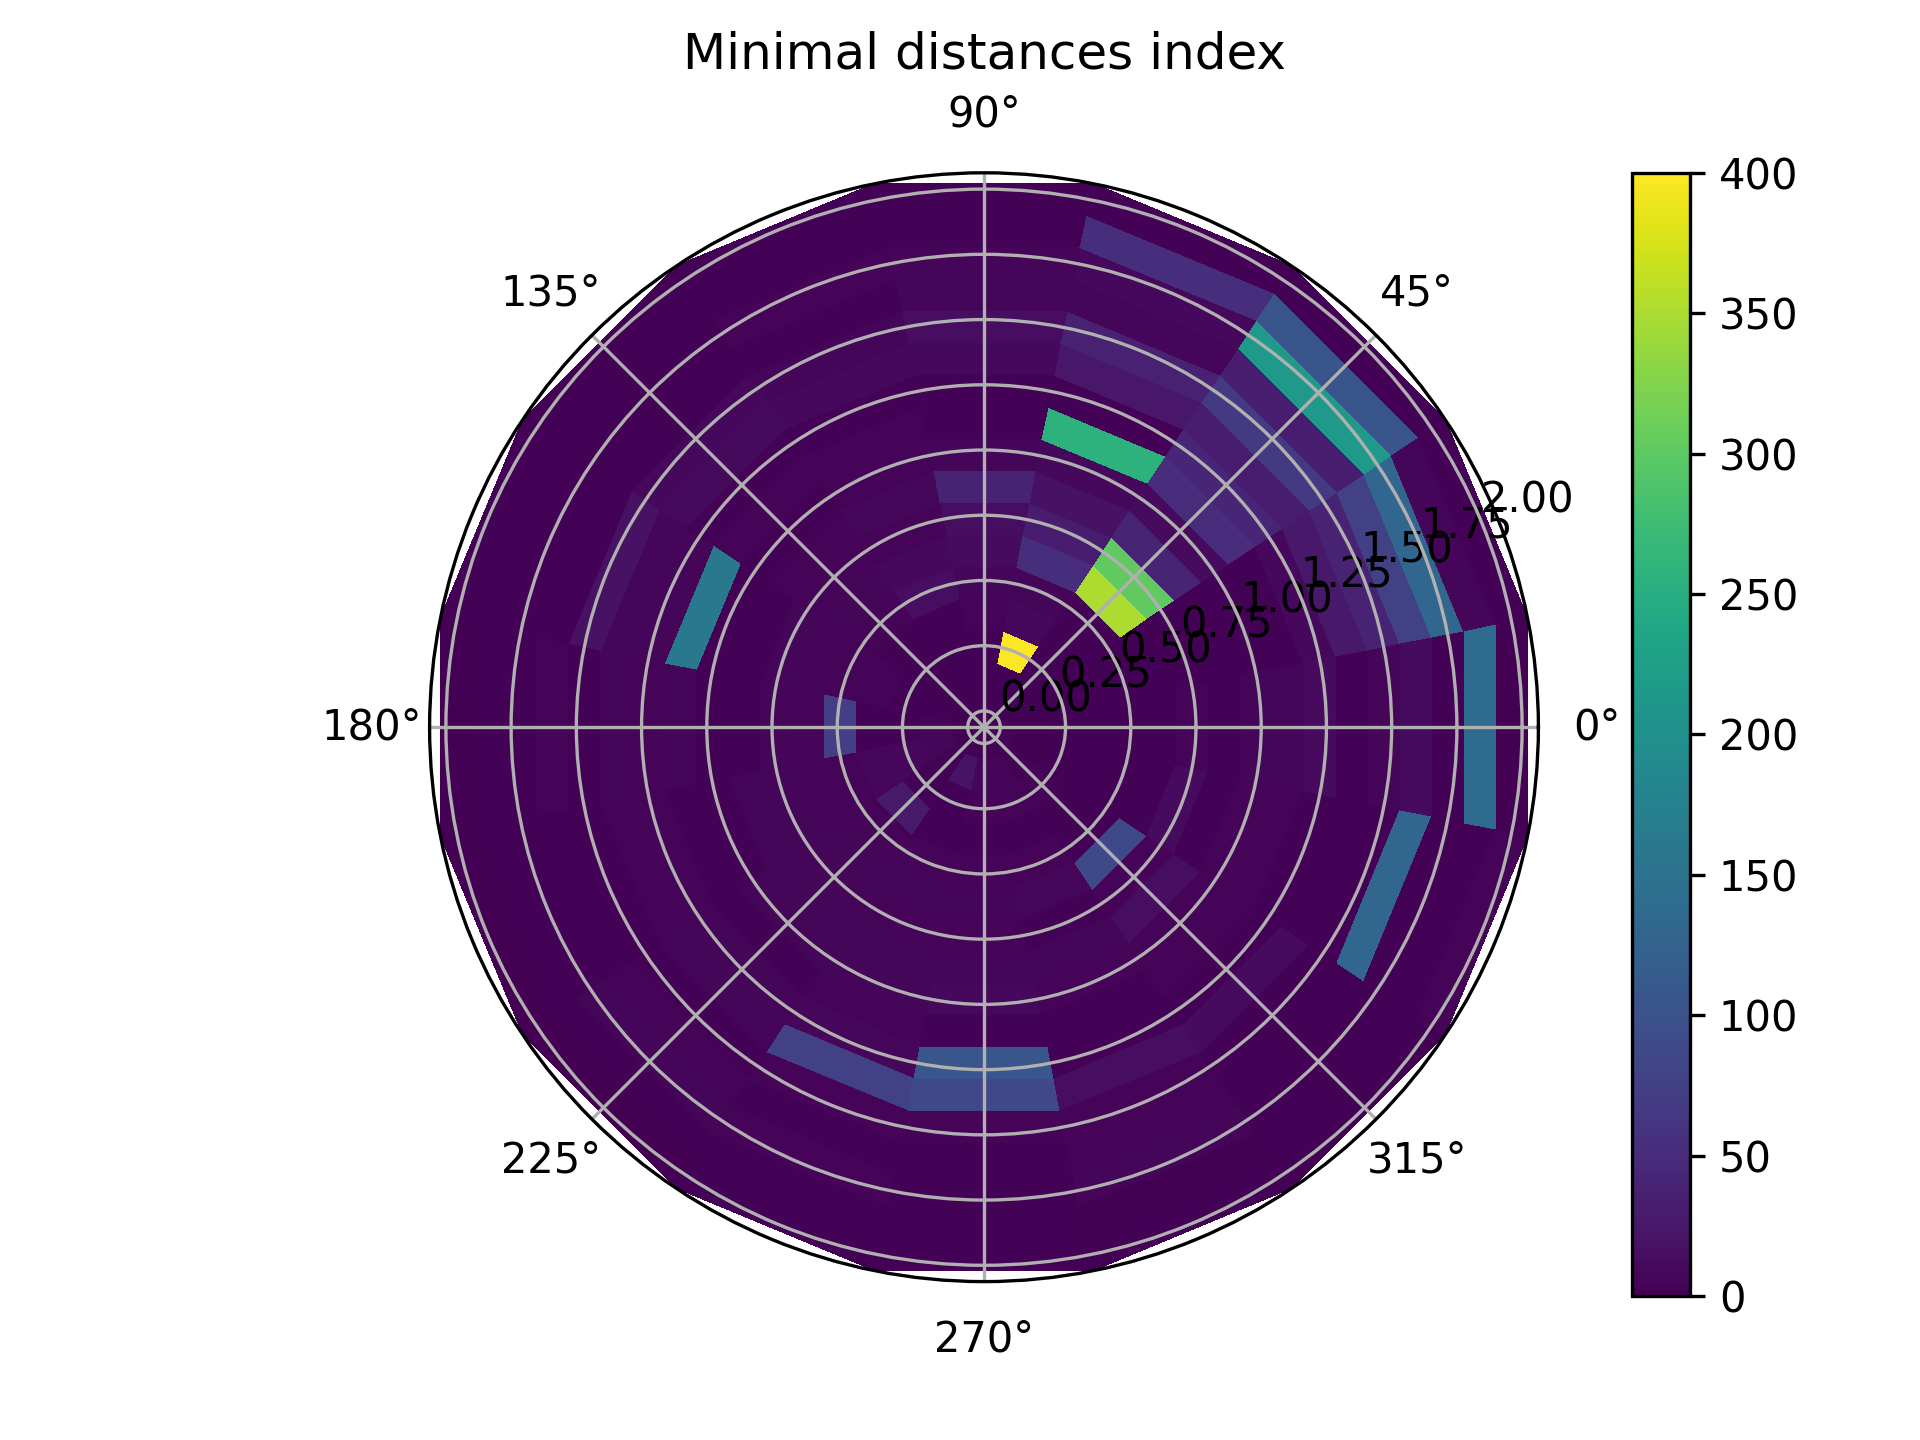
\includegraphics[width=0.31 \linewidth]{figures/experiments/Minimal_distances_index_baseline_2_1691621262_5000.png}
            \label{fig:SAC_baseline_min_distance_step/2}
            }
        \hfill
        \subfloat[$N = 5$]{
            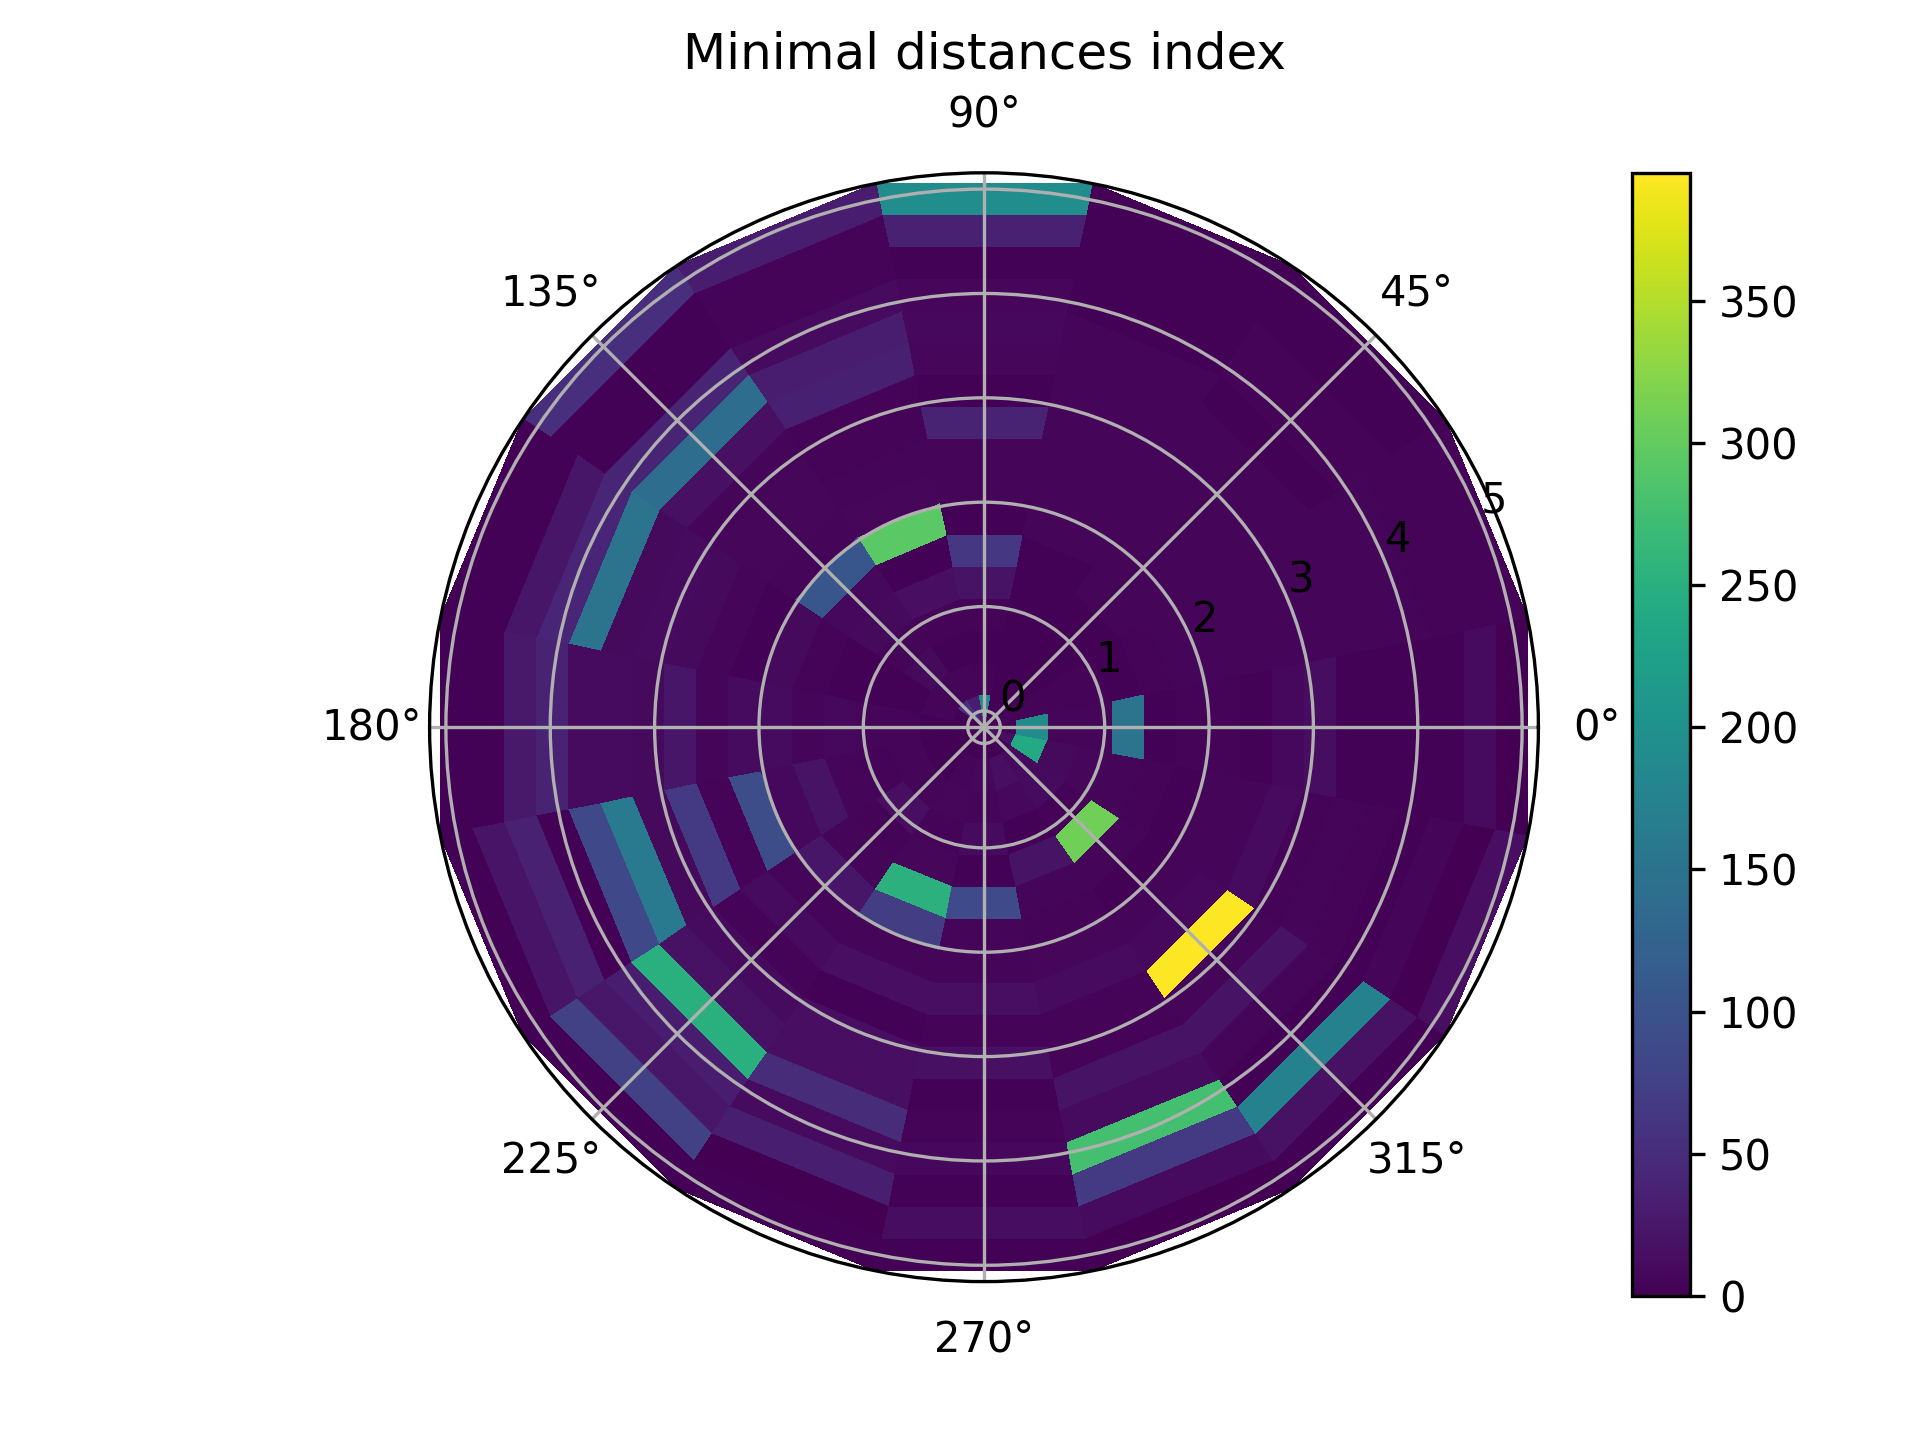
\includegraphics[width=0.31 \linewidth]{figures/experiments/Minimal_distances_index_baseline_5_1691621331_5000.png}
            \label{fig:SAC_baseline_min_distance_step/5}
            }
        \hfill
        \subfloat[$N = 10$]{
            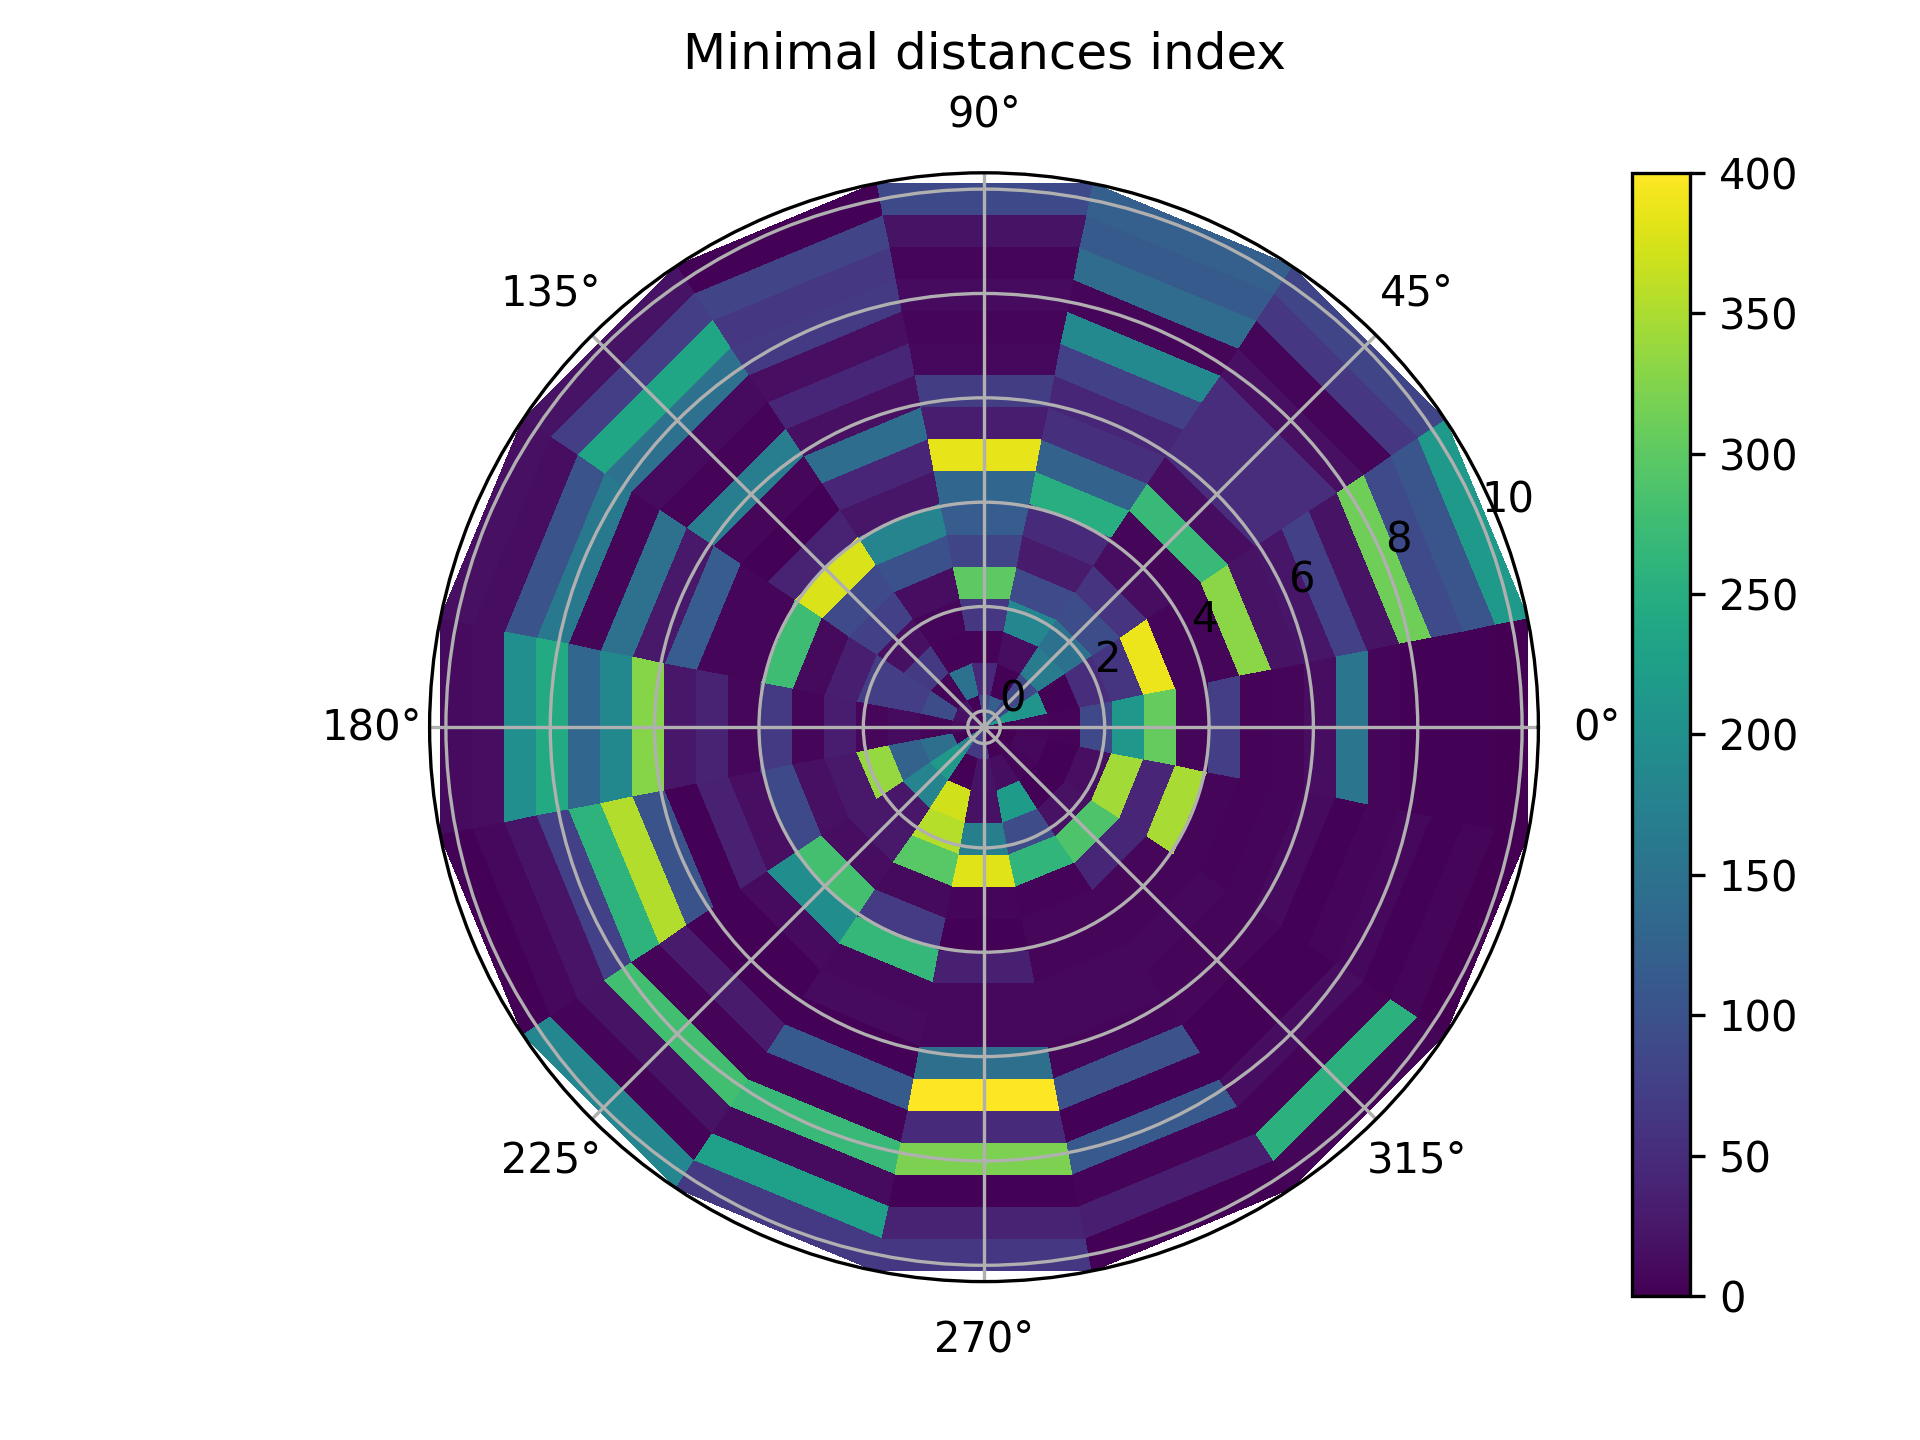
\includegraphics[width=0.31 \linewidth]{figures/experiments/Minimal_distances_index_baseline_10_1691618968_5000.png}
            \label{fig:SAC_baseline_min_distance_step/10}
            }
    \end{center}
    \caption[CCD iteration heatmap]{Heatmap of how many iterations CCD has needed to solve inverse kinematics starting from $[N, 0]$ targeting the middle of each polygon. The maximum budged are 20 times $N$ with a target precision of $0.1$.}
    \label{fig:SAC_baseline_min_distance_step}
\end{figure}

\section{Latent Model}

Moving on to the experiments to train a latent model. We train a latent model to augment SAC and let it control the latent model and therefor the actions from a higher level while having access to all state space information.

Since the standalone results of each latent model type are very similar I will discuss them together.
Both ways to train a model with the TargetGaussian Dataset yielded almost the same performance in the distance loss. This is not very surprising as we have seen neural networks struggle with the inverse Kinematics task while increasing the number of joints $N$. Looking deeper into the model performance shows that the distance loss is dependent is also dependent on the state information we are providing in datasets. \todo{think about how to plot this}   

We also have similar results with the imitation loss
\todo{big change in observation space distribution}


\section{SAC with Latent Model}

Embedding the Latent Model into the workflow of SAC yielded performances as presented in \chapref{chap:experiments}. While understanding and seeing the vast difference in problem solving strategies between the trained latent models and the Inverse Kinematics solver CCD it is quite surprising this approach works in the first place. Usually such a significant change in the observation space distribution, leads to unpredictable and unfeasible behavior in the predicted actions in the Action space. We tried to master this issue by introducing the imitation loss to emphasis predicted actions leading to state angles which are much closer to the original distribution. Arguments that the approach actually works can be found by looking into a greedy inference with the latent models where we simulate a very light weight version of the Plane-Robot-Environment while assuming the optimal policy, following the direction from start to end.

But why do we see differences for different latent dimensions? Looking first into those experiments with a latent dimension of 2. Since we are trying to encode the two dimensional target information which is sampled according to the idea of the TargetGaussianDataset, into a two dimensional gaussian manifold, the best information keeping strategy would be to pipe the mean values while returning a standard deviation close to zero. Because we do employ the ELBO with a gaussian distribution for a Variational Autoencoder we have to pick a parameterized latent distribution close the standard normal distribution. An additional difficulty is to encode the target position as independent random variables. Knowing these properties and constrains it could be quite challenging to compress. On the other hand choosing the latent dimension to high could add to much computational complexity, difficulty in sampling and a reduction in robustness.

As a result of the previous observations we can set the latent dimension of a VAE as an additional hyperparameter to optimize. Because setting it to high could lead the extremely high variance in the Soft Actor Critic task as shown in \figref{fig:SAC_latent_comparison/10} and setting it to low could lead to loss in encoded information. 

Further we want to revisit the action correlation plots. As previously mentioned the action correlation plots across all SAC experiments are vastly different from the initial distribution as in \figref{fig:dataset_action_correlation} but are very similar among themselves as in \figref{fig:SAC_action_correlation}. We can see the same hot-spots in left half across all SAC and SAC + VAE experiments which is clearly not a result to be expected because each models could chose a different solving strategy for itself and start each time from scratch. On the other hand activating the imitation loss in  the VAE experiements and merging this experiment with SAC should lead to a significant step towards the rhombus as in \figref{fig:dataset_action_correlation}. Instead the know hotspots as in \figref{fig:SAC_action_correlation} disappear and we get a new distribution with the same spike at the $[\pi, 0]$ shown in \figref{fig:SAC_action_correlation_comp/latent_4_imitation}.
